% AlohaMini Codebase Documentation
% LaTeX Beamer Presentation

\documentclass[aspectratio=169]{beamer}

% Theme settings
\usetheme{CambridgeUS}
\usecolortheme{default}

% Define darkred color for compatibility
\definecolor{darkred}{rgb}{0.55, 0.0, 0.0}

% Load common preamble
% AlohaMini Documentation - Common Preamble
% Beamer presentation with beaver theme

% ============================================
% PACKAGES
% ============================================

% TikZ for diagrams
\usepackage{tikz}
\usetikzlibrary{
    arrows.meta,
    shapes.geometric,
    shapes.misc,
    positioning,
    calc,
    fit,
    backgrounds,
    decorations.pathreplacing,
    chains
}

% Code listings
\usepackage{listings}
\usepackage{xcolor}

% Math
\usepackage{amsmath}
\usepackage{amssymb}

% Tables
\usepackage{booktabs}
\usepackage{array}
\usepackage{multirow}

% Graphics
\usepackage{graphicx}

% Hyperlinks
\usepackage{hyperref}

% Korean support (optional)
\usepackage{kotex}

% ============================================
% CODE LISTING STYLE
% ============================================

\definecolor{codegreen}{rgb}{0,0.6,0}
\definecolor{codegray}{rgb}{0.5,0.5,0.5}
\definecolor{codepurple}{rgb}{0.58,0,0.82}
\definecolor{backcolour}{rgb}{0.95,0.95,0.92}
\definecolor{codeblue}{rgb}{0.13,0.13,0.8}

\lstdefinestyle{pythonstyle}{
    backgroundcolor=\color{backcolour},
    commentstyle=\color{codegreen}\itshape,
    keywordstyle=\color{codeblue}\bfseries,
    numberstyle=\tiny\color{codegray},
    stringstyle=\color{codepurple},
    basicstyle=\ttfamily\tiny,
    breakatwhitespace=false,
    breaklines=true,
    captionpos=b,
    keepspaces=true,
    numbers=left,
    numbersep=3pt,
    showspaces=false,
    showstringspaces=false,
    showtabs=false,
    tabsize=2,
    language=Python,
    morekeywords={self, True, False, None, def, class, return, import, from, as, if, else, elif, for, while, try, except, finally, with, yield, lambda, and, or, not, in, is, pass, break, continue, raise, assert, global, nonlocal, async, await},
    frame=single,
    framerule=0.5pt,
    rulecolor=\color{codegray}
}

\lstset{style=pythonstyle}

% Inline code
\newcommand{\code}[1]{\texttt{\small #1}}
\newcommand{\pycode}[1]{\lstinline[language=Python]{#1}}

% ============================================
% TIKZ STYLES
% ============================================

\tikzstyle{module} = [
    rectangle,
    rounded corners=3pt,
    draw=darkred!80,
    fill=darkred!10,
    text width=2.5cm,
    minimum height=1cm,
    text centered,
    font=\small\bfseries
]

\tikzstyle{submodule} = [
    rectangle,
    rounded corners=2pt,
    draw=gray!60,
    fill=gray!10,
    text width=2cm,
    minimum height=0.7cm,
    text centered,
    font=\footnotesize
]

\tikzstyle{class} = [
    rectangle,
    draw=blue!60,
    fill=blue!10,
    text width=3cm,
    minimum height=0.8cm,
    text centered,
    font=\small\ttfamily
]

\tikzstyle{arrow} = [
    ->,
    >=stealth,
    thick,
    draw=darkred!70
]

\tikzstyle{flow} = [
    ->,
    >=Triangle,
    thick,
    draw=gray!70
]

\tikzstyle{joint} = [
    circle,
    draw=black,
    fill=orange!30,
    minimum size=0.4cm
]

\tikzstyle{link} = [
    line width=3pt,
    draw=gray!60
]

% ============================================
% CUSTOM COMMANDS
% ============================================

% File path styling
\newcommand{\filepath}[1]{\texttt{\color{codeblue}\small #1}}

% Highlight box
\newcommand{\highlight}[1]{%
    \colorbox{yellow!30}{\texttt{#1}}%
}

% Warning/Note boxes
\newenvironment{notebox}{%
    \begin{block}{Note}
}{%
    \end{block}
}

\newenvironment{warningbox}{%
    \begin{alertblock}{Warning}
}{%
    \end{alertblock}
}

% ============================================
% BEAMER CUSTOMIZATION
% ============================================

% Reduce text margins for more content space
\setbeamersize{text margin left=4mm, text margin right=4mm}

% Allow sloppy line breaking
\sloppy

% Tolerate small hbox/vbox overflows (up to 20pt for presentations)
\hfuzz=20pt
\vfuzz=20pt

% Frame title format (compact)
\setbeamertemplate{frametitle}{
    \vspace{0.3em}
    \insertframetitle
    \par
    \vspace{-0.4em}
    \textcolor{darkred!50}{\rule{\textwidth}{0.3pt}}
}

% Footer with page numbers
\setbeamertemplate{footline}{
    \leavevmode%
    \hbox{%
        \begin{beamercolorbox}[wd=.333333\paperwidth,ht=2.25ex,dp=1ex,left]{author in head/foot}%
            \usebeamerfont{author in head/foot}\hspace{1em}AlohaMini Documentation
        \end{beamercolorbox}%
        \begin{beamercolorbox}[wd=.333333\paperwidth,ht=2.25ex,dp=1ex,center]{title in head/foot}%
            \usebeamerfont{title in head/foot}\insertshorttitle
        \end{beamercolorbox}%
        \begin{beamercolorbox}[wd=.333333\paperwidth,ht=2.25ex,dp=1ex,right]{date in head/foot}%
            \usebeamerfont{date in head/foot}\insertframenumber{} / \inserttotalframenumber\hspace{1em}
        \end{beamercolorbox}%
    }%
    \vskip0pt%
}

% Remove navigation symbols
\setbeamertemplate{navigation symbols}{}

% Table of contents styling
\setbeamertemplate{section in toc}[sections numbered]
\setbeamertemplate{subsection in toc}[subsections numbered]


% ============================================
% DOCUMENT INFORMATION
% ============================================

\title[AlohaMini]{AlohaMini Codebase Documentation}
\subtitle{Dual-Arm Mobile Manipulation Robot}
\author{Technical Documentation}
\date{\today}
\institute{ManiSkill3 Integration}

% ============================================
% DOCUMENT BODY
% ============================================

\begin{document}

% Title slide
\begin{frame}
    \titlepage
\end{frame}

% Table of contents
\begin{frame}{Contents}
    \tableofcontents
\end{frame}

% ============================================
% SECTION 1: OVERVIEW
% ============================================
% 01_overview.tex - Project Overview
% AlohaMini Codebase Documentation

\section{Project Overview}

% ============================================
% SLIDE: Introduction
% ============================================
\begin{frame}{AlohaMini Robot}
\begin{columns}
\begin{column}{0.5\textwidth}
    \textbf{Dual-Arm Mobile Manipulation Robot}
    \vspace{0.5cm}

    \begin{itemize}
        \item 16 DOF total configuration
        \item Omnidirectional mobile base (3 wheels)
        \item Vertical lift mechanism
        \item Dual 6-DOF arms
        \item 5-camera perception system
    \end{itemize}
\end{column}
\begin{column}{0.5\textwidth}
    \centering
    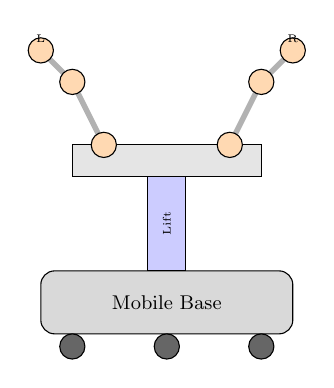
\begin{tikzpicture}[scale=0.8, transform shape]
        % Base
        \draw[fill=gray!30, rounded corners=5pt] (-2,-0.5) rectangle (2,0.5);
        \node at (0,0) {\small Mobile Base};

        % Wheels
        \draw[fill=black!60] (-1.5,-0.7) circle (0.2);
        \draw[fill=black!60] (1.5,-0.7) circle (0.2);
        \draw[fill=black!60] (0,-0.7) circle (0.2);

        % Lift
        \draw[fill=blue!20] (-0.3,0.5) rectangle (0.3,2);
        \node[rotate=90] at (0,1.25) {\tiny Lift};

        % Arm platform
        \draw[fill=gray!20] (-1.5,2) rectangle (1.5,2.5);

        % Left arm
        \draw[line width=2pt, gray!60] (-1,2.5) -- (-1.5,3.5) -- (-2,4);
        \node[joint] at (-1,2.5) {};
        \node[joint] at (-1.5,3.5) {};
        \node[joint] at (-2,4) {};
        \node[above] at (-2,4) {\tiny L};

        % Right arm
        \draw[line width=2pt, gray!60] (1,2.5) -- (1.5,3.5) -- (2,4);
        \node[joint] at (1,2.5) {};
        \node[joint] at (1.5,3.5) {};
        \node[joint] at (2,4) {};
        \node[above] at (2,4) {\tiny R};
    \end{tikzpicture}
\end{column}
\end{columns}
\end{frame}

% ============================================
% SLIDE: Robot Specifications
% ============================================
\begin{frame}{Robot Specifications}
\begin{table}
\centering
\begin{tabular}{lcc}
\toprule
\textbf{Component} & \textbf{DOF} & \textbf{Type} \\
\midrule
Mobile Base (X, Y, $\theta$) & 3 & Prismatic/Continuous \\
Vertical Lift & 1 & Prismatic \\
Left Arm & 6 & Revolute \\
Right Arm & 6 & Revolute \\
\midrule
\textbf{Total} & \textbf{16} & \\
\bottomrule
\end{tabular}
\end{table}

\vspace{0.5cm}

\begin{block}{Action Space (ManiSkill3)}
\texttt{[base\_x, base\_y, base\_rot, lift, left\_arm(6), right\_arm(6)]}
\end{block}
\end{frame}

% ============================================
% SLIDE: Software Stack
% ============================================
\begin{frame}{Software Stack}
\centering
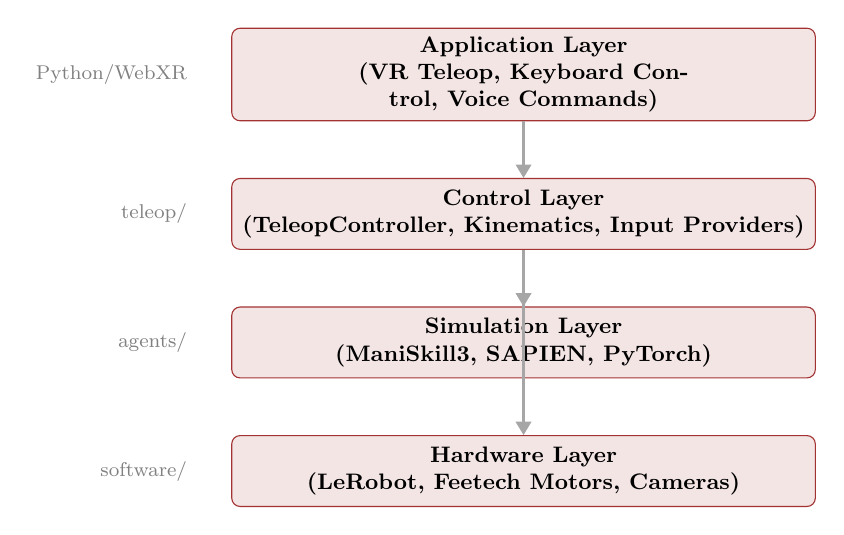
\begin{tikzpicture}[node distance=0.8cm, scale=0.9, transform shape]
    % Stack layers
    \node[module, text width=8cm, minimum height=1cm] (app) at (0,0)
        {Application Layer\\(VR Teleop, Keyboard Control, Voice Commands)};

    \node[module, text width=8cm, minimum height=1cm, below=of app] (ctrl)
        {Control Layer\\(TeleopController, Kinematics, Input Providers)};

    \node[module, text width=8cm, minimum height=1cm, below=of ctrl] (sim)
        {Simulation Layer\\(ManiSkill3, SAPIEN, PyTorch)};

    \node[module, text width=8cm, minimum height=1cm, below=of sim] (hw)
        {Hardware Layer\\(LeRobot, Feetech Motors, Cameras)};

    % Arrows
    \draw[flow] (app) -- (ctrl);
    \draw[flow] (ctrl) -- (sim);
    \draw[flow] (ctrl) -- (hw);

    % Side labels
    \node[left=0.5cm of app, font=\footnotesize, text=gray] {Python/WebXR};
    \node[left=0.5cm of ctrl, font=\footnotesize, text=gray] {teleop/};
    \node[left=0.5cm of sim, font=\footnotesize, text=gray] {agents/};
    \node[left=0.5cm of hw, font=\footnotesize, text=gray] {software/};
\end{tikzpicture}
\end{frame}

% ============================================
% SLIDE: Key Features
% ============================================
\begin{frame}{Key Features}
\begin{columns}[t]
\begin{column}{0.5\textwidth}
    \textbf{Simulation (ManiSkill3)}
    \begin{itemize}
        \item GPU-accelerated physics
        \item Virtual mobile base
        \item Grasping detection
        \item Camera rendering
        \item ReplicaCAD scenes
    \end{itemize}

    \vspace{0.3cm}

    \textbf{Teleoperation}
    \begin{itemize}
        \item Keyboard control (XLeRobot-style)
        \item VR control (WebXR)
        \item 50 Hz control loop
        \item IK-based arm control
    \end{itemize}
\end{column}
\begin{column}{0.5\textwidth}
    \textbf{Physical Robot}
    \begin{itemize}
        \item LeRobot integration
        \item 5-camera perception
        \item Trajectory recording
        \item Voice commands
    \end{itemize}

    \vspace{0.3cm}

    \textbf{ROS Simulation}
    \begin{itemize}
        \item RViz visualization
        \item Gazebo physics
        \item URDF models
        \item ROS1/ROS2 support
    \end{itemize}
\end{column}
\end{columns}
\end{frame}

% ============================================
% SLIDE: Code Metrics
% ============================================
\begin{frame}{Code Metrics}
\begin{columns}
\begin{column}{0.5\textwidth}
    \begin{table}
    \centering
    \begin{tabular}{lr}
    \toprule
    \textbf{Module} & \textbf{Lines} \\
    \midrule
    agents/aloha\_mini & $\sim$850 \\
    teleop/ & $\sim$2,000 \\
    kinematics/ & $\sim$800 \\
    software/ (LeRobot) & $\sim$1,500 \\
    \midrule
    \textbf{Total} & $\sim$5,150 \\
    \bottomrule
    \end{tabular}
    \end{table}
\end{column}
\begin{column}{0.5\textwidth}
    \textbf{Key Classes}
    \begin{itemize}
        \item \code{AlohaMiniVirtual}
        \item \code{TeleopController}
        \item \code{AlohaMiniKinematics}
        \item \code{ControlGoal}
        \item \code{KeyboardController}
        \item \code{VRControllerServer}
    \end{itemize}
\end{column}
\end{columns}
\end{frame}


% ============================================
% SECTION 2: AGENTS MODULE
% ============================================
% 02_agents.tex - Robot Agents Module
% AlohaMini Codebase Documentation

\section{Agents Module}

% ============================================
% SLIDE: Module Overview
% ============================================
\begin{frame}{agents/aloha\_mini/ Module}
\begin{columns}
\begin{column}{0.45\textwidth}
    \textbf{Purpose:} Define robot agents for ManiSkill3 simulation

    \vspace{0.3cm}

    \textbf{Files:}
    \begin{itemize}
        \item \filepath{base\_agent.py} (208 lines)
        \item \filepath{aloha\_mini\_so100\_v2.py} (351 lines)
        \item \filepath{\_\_init\_\_.py}
    \end{itemize}
\end{column}
\begin{column}{0.55\textwidth}
    \centering
    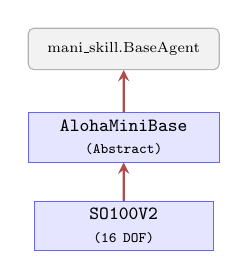
\begin{tikzpicture}[scale=0.75, transform shape]
        % ManiSkill BaseAgent (top)
        \node[submodule, text width=3cm] (maniskill) at (0,3) {\scriptsize mani\_skill.BaseAgent};

        % AlohaMiniBase (middle)
        \node[class, text width=3cm] (base) at (0,1.5) {
            \textbf{AlohaMiniBase}\\
            \scriptsize (Abstract)
        };

        % SO100V2 (bottom)
        \node[class, text width=2.8cm] (so100) at (0,0) {
            SO100V2\\
            \scriptsize (16 DOF)
        };

        % Inheritance arrows - directly connected
        \draw[arrow] (base) -- (maniskill);
        \draw[arrow] (so100) -- (base);
    \end{tikzpicture}
\end{column}
\end{columns}
\end{frame}

% ============================================
% SLIDE: base_agent.py Overview
% ============================================
\begin{frame}[fragile]{base\_agent.py - Base Class}
\begin{columns}
\begin{column}{0.5\textwidth}
\begin{lstlisting}[basicstyle=\ttfamily\scriptsize]
class AlohaMiniBaseAgent(BaseAgent):
    """Base agent for variants."""
    BASE_JOINT_NAMES = [
        "root_x_axis_joint",
        "root_y_axis_joint",
        "root_z_rotation_joint",
    ]
    LIFT_JOINT_NAMES = ["vertical_move"]

    @abstractmethod
    def get_left_ee_pose(self): pass

    @abstractmethod
    def get_right_ee_pose(self): pass
\end{lstlisting}
\end{column}
\begin{column}{0.5\textwidth}
    \textbf{Common Functionality:}
    \begin{itemize}
        \item Joint name definitions
        \item Controller parameter defaults
        \item \code{\_create\_base\_controller()}
        \item \code{is\_grasping()} (Template Method)
        \item \code{is\_static()}
    \end{itemize}

    \vspace{0.2cm}

    \begin{block}{Design Pattern}
    \footnotesize\textbf{Template Method}: \code{is\_grasping()} calls abstract \code{\_check\_single\_arm\_grasping()}
    \end{block}
\end{column}
\end{columns}
\end{frame}

% ============================================
% SLIDE: Controller Helper Methods
% ============================================
\begin{frame}[fragile]{base\_agent.py - Controller Helpers}
\begin{lstlisting}
def _create_base_controller(self):
    """Create PDBaseVelController for virtual mobile base."""
    return PDBaseVelControllerConfig(
        self.base_joint_names,
        lower=[-1, -1, -3.14],    # [vx, vy, omega]
        upper=[1, 1, 3.14],
        damping=self.base_damping,        # 1000
        force_limit=self.base_force_limit, # 500
    )

def _create_lift_pos_controller(self):
    """Create position controller for lift mechanism."""
    return PDJointPosControllerConfig(
        self.lift_joint_names,
        stiffness=self.lift_stiffness,    # 2e3
        damping=self.lift_damping,        # 2e2
        force_limit=self.lift_force_limit, # 150
        normalize_action=False,
    )
\end{lstlisting}
\end{frame}

% ============================================
% SLIDE: is_grasping Template Method
% ============================================
\begin{frame}[fragile]{base\_agent.py - Grasping Detection}
\begin{lstlisting}
def is_grasping(self, object: Actor, min_force=0.5,
                max_angle=110, arm_id=None):
    """Check if robot is grasping an object."""
    if arm_id is None:
        # Check both arms
        arm1 = self._check_single_arm_grasping(
            object, min_force, max_angle, arm_id=1)
        arm2 = self._check_single_arm_grasping(
            object, min_force, max_angle, arm_id=2)
        return torch.logical_or(arm1, arm2)
    else:
        return self._check_single_arm_grasping(
            object, min_force, max_angle, arm_id)

@abstractmethod
def _check_single_arm_grasping(self, object, ...):
    """Implemented by subclass (different gripper structures)"""
    pass
\end{lstlisting}

\begin{block}{Note}
Different gripper structures require different contact force calculations.
\end{block}
\end{frame}

% ============================================
% SLIDE: aloha_mini_so100_v2.py Overview
% ============================================
\begin{frame}{aloha\_mini\_so100\_v2.py - SO100 Variant}
\begin{columns}
\begin{column}{0.5\textwidth}
    \textbf{Configuration:}
    \begin{itemize}
        \item \code{uid = "aloha\_mini\_so100\_v2"}
        \item Virtual base (prismatic X/Y)
        \item 16 DOF total
        \item SO100 arm design
    \end{itemize}

    \vspace{0.3cm}

    \textbf{Joint Names:}
    \begin{itemize}
        \item \code{left\_shoulder\_pan/lift}
        \item \code{elbow\_flex}, \code{wrist\_flex}
        \item \code{wrist\_roll}, \code{gripper}
    \end{itemize}
\end{column}
\begin{column}{0.5\textwidth}
    \textbf{Controller Parameters:}
    \begin{table}
    \centering
    \footnotesize
    \begin{tabular}{lr}
    \toprule
    \textbf{Parameter} & \textbf{Value} \\
    \midrule
    arm\_stiffness & 3e3 \\
    arm\_damping & 2e2 \\
    arm\_force\_limit & 100 N \\
    gripper\_stiffness & 100 \\
    \bottomrule
    \end{tabular}
    \end{table}

    \vspace{0.3cm}

    \textbf{Cameras:}
    \begin{itemize}
        \item cam\_main (320$\times$240)
        \item cam\_left\_wrist (128$\times$128)
        \item cam\_right\_wrist (128$\times$128)
    \end{itemize}
\end{column}
\end{columns}
\end{frame}

% ============================================
% SLIDE: Keyframes
% ============================================
\begin{frame}[fragile]{Keyframes Configuration}
\begin{lstlisting}[basicstyle=\ttfamily\scriptsize]
keyframes = dict(
    rest=Keyframe(
        qpos=np.array([
            0.0, 0.0, 0.0,  # Base: x, y, rotation
            0.0,            # Lift
            0.0, 0.0, 0.0, 0.0, 0.0, 0.0,  # Left arm
            0.0, 0.0, 0.0, 0.0, 0.0, 0.0,  # Right arm
        ]),
        pose=sapien.Pose(p=[0, 0, 0]),
    ),
    ready=Keyframe(
        qpos=np.array([
            0.0, 0.0, 0.0, 0.05,           # base + lift
            0.0, 0.3, -0.3, 0.0, 0.3, 0.0, # left
            0.0, 0.3, -0.3, 0.0, 0.3, 0.0, # right
        ]),
    ),
)
\end{lstlisting}
\end{frame}

% ============================================
% SLIDE: Camera Configuration
% ============================================
\begin{frame}[fragile]{Camera Setup}
\begin{lstlisting}[basicstyle=\ttfamily\scriptsize]
@property
def _sensor_configs(self):
    q_main = euler_to_quat_xyz(
        math.radians(90), math.radians(90), 0)  # overhead
    q_wrist = euler_to_quat_xyz(
        0, math.radians(45), math.radians(-90)) # 45deg down

    return [
        CameraConfig(uid="cam_main",
            pose=Pose.create_from_pq(p=[0.0, 0.0, 1.45], q=q_main),
            width=320, height=240, fov=1.5, entity_uid="base_link"),
        CameraConfig(uid="cam_left_wrist",
            pose=Pose.create_from_pq(p=[0.0, 0.0, 0.15], q=q_wrist),
            width=128, height=128, fov=1.3, entity_uid="left_link4"),
    ]
\end{lstlisting}
\end{frame}

% ============================================
% SLIDE: SO100 Grasping Detection
% ============================================
\begin{frame}[fragile]{Grasping Detection}
\begin{lstlisting}
def _check_single_arm_grasping(self, object, min_force=0.5,
                                max_angle=110, arm_id=1):
    """SO100 style: two-finger grasping detection."""
    finger1_link = self.left_finger1_link  # Fixed_Jaw
    finger2_link = self.left_finger2_link  # Moving_Jaw

    l_contact = self.scene.get_pairwise_contact_forces(
        finger1_link, object)
    r_contact = self.scene.get_pairwise_contact_forces(
        finger2_link, object)

    lforce = torch.linalg.norm(l_contact, axis=1)
    rforce = torch.linalg.norm(r_contact, axis=1)

    # Direction to open gripper
    ldirection = finger1_link.pose.to_transformation_matrix()[..., :3, 1]
    rdirection = -finger2_link.pose.to_transformation_matrix()[..., :3, 1]

    # Check force and angle thresholds
    lflag = (lforce >= min_force) & (angle <= max_angle)
    rflag = (rforce >= min_force) & (angle <= max_angle)
    return torch.logical_and(lflag, rflag)
\end{lstlisting}
\end{frame}

% ============================================
% SLIDE: Class Diagram Summary
% ============================================
\begin{frame}{Agents Module - Class Diagram}
\centering
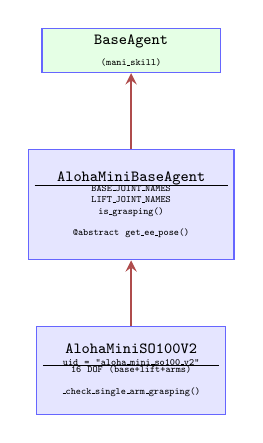
\begin{tikzpicture}[scale=0.7, transform shape]
    % BaseAgent from ManiSkill
    \node[class, text width=3cm, fill=green!10] (base) at (0,5) {
        \footnotesize\textbf{BaseAgent}\\
        \tiny (mani\_skill)
    };

    % AlohaMiniBaseAgent
    \node[class, text width=3.5cm, minimum height=2cm] (aloha) at (0,2.2) {
        \footnotesize\textbf{AlohaMiniBaseAgent}\\
        \hrule
        \tiny BASE\_JOINT\_NAMES\\
        \tiny LIFT\_JOINT\_NAMES\\
        \tiny is\_grasping()\\
        \tiny @abstract get\_ee\_pose()
    };

    % AlohaMiniSO100V2
    \node[class, text width=3.2cm, minimum height=1.6cm] (so100) at (0,-0.8) {
        \footnotesize\textbf{AlohaMiniSO100V2}\\
        \tiny uid = "aloha\_mini\_so100\_v2"\\
        \hrule
        \tiny 16 DOF (base+lift+arms)\\
        \tiny \_check\_single\_arm\_grasping()
    };

    % Arrows
    \draw[arrow] (aloha) -- (base);
    \draw[arrow] (so100) -- (aloha);
\end{tikzpicture}
\end{frame}


% ============================================
% SECTION 3: TELEOPERATION MODULE
% ============================================
% 03_teleop.tex - Teleoperation Module
% AlohaMini Codebase Documentation

\section{Teleoperation Module}

% ============================================
% SLIDE: Module Overview
% ============================================
\begin{frame}{teleop/ Module Overview}
\begin{columns}
\begin{column}{0.4\textwidth}
    \textbf{Purpose:} Real-time teleoperation from keyboard/VR input to ManiSkill3 actions

    \vspace{0.3cm}

    \textbf{Key Files:}
    \begin{itemize}
        \item \filepath{controller.py}
        \item \filepath{config.py}
        \item \filepath{inputs/base.py}
        \item \filepath{inputs/keyboard\_controller.py}
        \item \filepath{inputs/vr\_ws\_server.py}
    \end{itemize}
\end{column}
\begin{column}{0.6\textwidth}
    \centering
    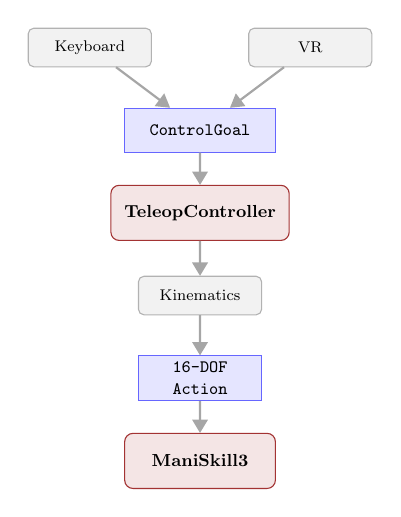
\begin{tikzpicture}[scale=0.7, transform shape]
        % Input sources
        \node[submodule] (keyboard) at (-2, 3) {Keyboard};
        \node[submodule] (vr) at (2, 3) {VR};

        % ControlGoal
        \node[class, text width=2.5cm] (goal) at (0, 1.5) {ControlGoal};

        % Controller
        \node[module, text width=3cm] (ctrl) at (0, 0) {TeleopController};

        % Kinematics
        \node[submodule] (ik) at (0, -1.5) {Kinematics};

        % Action
        \node[class, text width=2cm] (action) at (0, -3) {16-DOF Action};

        % ManiSkill
        \node[module, text width=2.5cm] (env) at (0, -4.5) {ManiSkill3};

        % Arrows
        \draw[flow] (keyboard) -- (goal);
        \draw[flow] (vr) -- (goal);
        \draw[flow] (goal) -- (ctrl);
        \draw[flow] (ctrl) -- (ik);
        \draw[flow] (ik) -- (action);
        \draw[flow] (action) -- (env);
    \end{tikzpicture}
\end{column}
\end{columns}
\end{frame}

% ============================================
% SLIDE: Data Structures - ControlGoal
% ============================================
\begin{frame}[fragile]{inputs/base.py - ControlGoal}
\begin{lstlisting}
@dataclass
class ControlGoal:
    """Command message from input provider to controller."""

    # Target position in normalized space
    left_target: Optional[np.ndarray] = None   # [x, y, z]
    right_target: Optional[np.ndarray] = None  # [x, y, z]

    # Direct joint angle targets (radians)
    left_joint_angles: Optional[np.ndarray] = None  # 6 joints
    right_joint_angles: Optional[np.ndarray] = None

    # Gripper state
    left_gripper_closed: bool = False
    right_gripper_closed: bool = False

    # Control mode
    mode: ControlMode = ControlMode.IDLE

    # Mobile base velocity
    base_velocity: Optional[np.ndarray] = None  # [vx, vy, omega]

    # Lift delta
    lift_delta: float = 0.0
\end{lstlisting}
\end{frame}

% ============================================
% SLIDE: Data Structures - ArmState
% ============================================
\begin{frame}[fragile]{inputs/base.py - ArmState}
\begin{lstlisting}[basicstyle=\ttfamily\scriptsize]
@dataclass
class ArmState:
    """Internal state tracking for one arm."""
    ee_pos: np.ndarray        # [y, z] in arm plane
    joint_angles: np.ndarray  # 6 joints (radians)
    pitch: float = 0.0        # Elbow angle sum
    gripper_closed: bool = False
    target_pos: Optional[np.ndarray] = None
\end{lstlisting}

\vspace{0.2cm}

\begin{block}{Coordinate System}
\begin{itemize}
    \item \code{ee\_y}: Forward direction (usually negative at home)
    \item \code{ee\_z}: Height (positive = up)
\end{itemize}
\end{block}
\end{frame}

% ============================================
% SLIDE: ControlMode Enum
% ============================================
\begin{frame}[fragile]{inputs/base.py - ControlMode}
\begin{lstlisting}
class ControlMode(Enum):
    """Control mode for teleoperation."""

    IDLE = "idle"           # No active control
    POSITION = "position"   # Position control (IK-based)
    VELOCITY = "velocity"   # Velocity control (direct joint)
\end{lstlisting}

\vspace{0.5cm}

\begin{table}
\centering
\begin{tabular}{lll}
\toprule
\textbf{Mode} & \textbf{Input} & \textbf{Processing} \\
\midrule
IDLE & None & Hold current position \\
POSITION & Target [x,y,z] & IK solver computes joints \\
VELOCITY & Joint deltas & Direct joint angle update \\
\bottomrule
\end{tabular}
\end{table}
\end{frame}

% ============================================
% SLIDE: TeleopController Overview
% ============================================
\begin{frame}{controller.py - TeleopController}
\begin{columns}
\begin{column}{0.5\textwidth}
    \textbf{Responsibilities:}
    \begin{itemize}
        \item Process keyboard/VR input
        \item Compute IK for both arms
        \item Generate 16-DOF action array
        \item Track arm states
        \item Handle mobile base control
    \end{itemize}

    \vspace{0.3cm}

    \textbf{Key Methods:}
    \begin{itemize}
        \item \code{process\_goal()}
        \item \code{compute\_action()}
        \item \code{update\_arm\_state()}
        \item \code{get\_action()}
    \end{itemize}
\end{column}
\begin{column}{0.5\textwidth}
    \textbf{State Variables:}
    \begin{itemize}
        \item \code{left\_arm\_state: ArmState}
        \item \code{right\_arm\_state: ArmState}
        \item \code{current\_lift: float}
        \item \code{kinematics: AlohaMiniKinematics}
    \end{itemize}

    \vspace{0.3cm}

    \textbf{Configuration:}
    \begin{itemize}
        \item Control frequency: 50 Hz
        \item Position step: 4mm
        \item Angle step: $1^{\circ}$
    \end{itemize}
\end{column}
\end{columns}
\end{frame}

% ============================================
% SLIDE: TeleopController - process_goal
% ============================================
\begin{frame}[fragile,shrink=3]{controller.py - process\_goal()}
\begin{lstlisting}
def process_goal(self, goal: ControlGoal):
    """Process a control goal and update internal state."""

    # Handle mobile base velocity
    if goal.base_velocity is not None:
        self.base_velocity = goal.base_velocity

    # Handle lift
    if goal.lift_delta != 0:
        self.current_lift += goal.lift_delta
        self.current_lift = np.clip(
            self.current_lift, 0.0, 0.6)  # 0-60cm

    # Handle left arm
    if goal.left_target is not None:
        self._update_arm_from_target(
            self.left_arm_state, goal.left_target)
    elif goal.left_joint_angles is not None:
        self.left_arm_state.joint_angles = goal.left_joint_angles

    # Handle gripper
    self.left_arm_state.gripper_closed = goal.left_gripper_closed

    # Similar for right arm...
\end{lstlisting}
\end{frame}

% ============================================
% SLIDE: TeleopController - compute_action
% ============================================
\begin{frame}[fragile]{controller.py - compute\_action()}
\begin{lstlisting}[basicstyle=\ttfamily\scriptsize]
def compute_action(self) -> np.ndarray:
    """Generate 16-DOF action array for ManiSkill3."""
    action = np.zeros(16)
    action[0:3] = self.base_velocity     # [vx, vy, omega]
    action[3] = self.current_lift        # Lift position
    action[4:10] = self.left_arm_state.joint_angles   # Left arm
    action[10:16] = self.right_arm_state.joint_angles # Right arm
    return action
\end{lstlisting}

\begin{block}{Action Space Layout}
\small\texttt{[vx, vy, omega, lift, L1..L6, R1..R6]}
\end{block}
\end{frame}

% ============================================
% SLIDE: Keyboard Controller
% ============================================
\begin{frame}{inputs/keyboard\_controller.py}
\begin{columns}
\begin{column}{0.5\textwidth}
    \textbf{Left Arm Keys:}
    \begin{table}
    \centering
    \footnotesize
    \begin{tabular}{ll}
    \toprule
    \textbf{Keys} & \textbf{Action} \\
    \midrule
    Q/A & Joint 1 (+/-) \\
    W/S & Joint 2 (+/-) \\
    E/D & Joint 3 (+/-) \\
    R/F & Joint 4 (+/-) \\
    T/G & Joint 5 (+/-) \\
    Y/H & Gripper \\
    \bottomrule
    \end{tabular}
    \end{table}
\end{column}
\begin{column}{0.5\textwidth}
    \textbf{Right Arm Keys:}
    \begin{table}
    \centering
    \footnotesize
    \begin{tabular}{ll}
    \toprule
    \textbf{Keys} & \textbf{Action} \\
    \midrule
    U/J & Joint 1 (+/-) \\
    I/K & Joint 2 (+/-) \\
    O/L & Joint 3 (+/-) \\
    P/; & Joint 4 (+/-) \\
    {[}/' & Joint 5 (+/-) \\
    {]}/\textbackslash & Gripper \\
    \bottomrule
    \end{tabular}
    \end{table}
\end{column}
\end{columns}

\vspace{0.3cm}

\textbf{Mobile Base:} Numpad 8/5 (forward/back), 4/6 (left/right), 7/9 (rotate)

\textbf{Lift:} PageUp/PageDown
\end{frame}

% ============================================
% SLIDE: Keyboard Controller Code
% ============================================
\begin{frame}[fragile]{keyboard\_controller.py - Key Processing}
\begin{lstlisting}
def process_input(self, keys) -> ControlGoal:
    """Process pygame key states to ControlGoal."""

    goal = ControlGoal(mode=ControlMode.VELOCITY)
    joint_deltas = np.zeros(6)

    # Left arm joint control
    if keys[pygame.K_q]: joint_deltas[0] += self.angle_step
    if keys[pygame.K_a]: joint_deltas[0] -= self.angle_step
    if keys[pygame.K_w]: joint_deltas[1] += self.angle_step
    if keys[pygame.K_s]: joint_deltas[1] -= self.angle_step
    # ... more joints

    # Apply deltas to current state
    goal.left_joint_angles = self.current_left + joint_deltas

    # Mobile base
    base_vel = np.zeros(3)
    if keys[pygame.K_KP8]: base_vel[0] = 0.3  # forward
    if keys[pygame.K_KP5]: base_vel[0] = -0.3 # backward
    goal.base_velocity = base_vel

    return goal
\end{lstlisting}
\end{frame}

% ============================================
% SLIDE: VR WebSocket Server
% ============================================
\begin{frame}{inputs/vr\_ws\_server.py - VR Interface}
\begin{columns}
\begin{column}{0.5\textwidth}
    \textbf{Features:}
    \begin{itemize}
        \item WebXR controller input
        \item HTTPS + WebSocket Secure
        \item Real-time camera streaming
        \item Pose-to-IK conversion
    \end{itemize}

    \vspace{0.2cm}

    \textbf{Protocol:}
    \begin{enumerate}
        \item Client connects via WSS
        \item Sends controller poses (JSON)
        \item Server converts to ControlGoal
        \item Streams camera frames back
    \end{enumerate}
\end{column}
\begin{column}{0.5\textwidth}
    \centering
    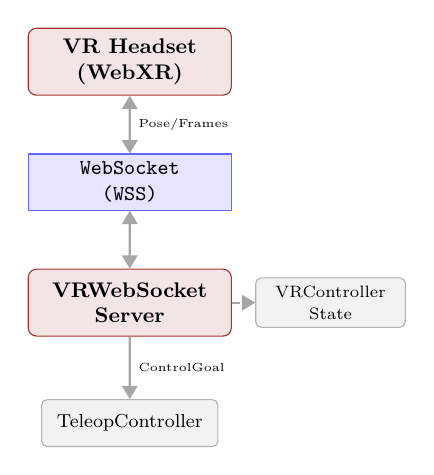
\begin{tikzpicture}[scale=0.85, transform shape]
        % VR Headset
        \node[module, text width=2.8cm] (vr) at (0, 3) {VR Headset\\(WebXR)};

        % WebSocket
        \node[class, text width=2.8cm] (ws) at (0, 1.2) {WebSocket\\(WSS)};

        % Server
        \node[module, text width=2.8cm] (server) at (0, -0.6) {VRWebSocket\\Server};

        % Controller State - moved to right side
        \node[submodule, text width=2cm] (state) at (3, -0.6) {\scriptsize VRController\\State};

        % Controller
        \node[submodule, text width=2.4cm] (ctrl) at (0, -2.4) {TeleopController};

        % Arrows
        \draw[flow, <->] (vr) -- node[right, font=\tiny] {Pose/Frames} (ws);
        \draw[flow, <->] (ws) -- (server);
        \draw[flow, dashed] (server) -- (state);
        \draw[flow] (server) -- node[right, font=\tiny] {ControlGoal} (ctrl);
    \end{tikzpicture}
\end{column}
\end{columns}
\end{frame}

% ============================================
% SLIDE: VR Message Format
% ============================================
\begin{frame}[fragile]{vr\_ws\_server.py - Message Format}
\begin{lstlisting}
# Incoming VR controller message
{
    "type": "controller_update",
    "left": {
        "position": [x, y, z],      # World coordinates
        "rotation": [qx, qy, qz, qw],
        "buttons": {
            "trigger": 0.8,         # Gripper control
            "grip": true
        }
    },
    "right": { ... },
    "head": {
        "position": [x, y, z],
        "rotation": [qx, qy, qz, qw]
    }
}
\end{lstlisting}

\begin{block}{Scaling}
VR positions are scaled by \code{vr\_position\_scale\_xy = 0.7} before IK
\end{block}
\end{frame}

% ============================================
% SLIDE: config.py
% ============================================
\begin{frame}[fragile,shrink=3]{config.py - TeleopConfig}
\begin{lstlisting}
@dataclass
class TeleopConfig:
    """Teleoperation configuration."""

    # Network settings
    host_ip: str = "0.0.0.0"
    ws_port: int = 8765
    https_port: int = 8443

    # SSL certificates
    cert_file: str = "cert.pem"
    key_file: str = "key.pem"

    # Control parameters
    control_freq: int = 50       # Hz
    pos_step: float = 0.004      # 4mm per step
    angle_step: float = 1.0      # 1 degree per step

    # IK parameters (from URDF)
    l1: float = 0.116            # Upper arm length
    l2: float = 0.134            # Lower arm length

    # VR scaling
    vr_position_scale_xy: float = 0.7
    vr_position_scale_z: float = 1.0
\end{lstlisting}
\end{frame}

% ============================================
% SLIDE: Teleop Flow Diagram
% ============================================
\begin{frame}[shrink=5]{Teleoperation Data Flow}
\centering
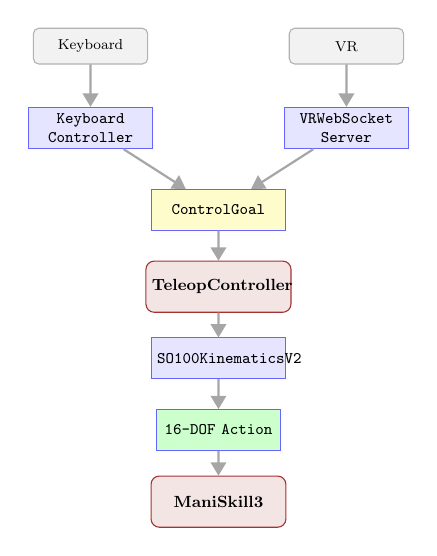
\begin{tikzpicture}[scale=0.65, transform shape, node distance=0.8cm]
    % Input layer
    \node[submodule, text width=2cm] (kbd) at (-2.5, 3.2) {Keyboard};
    \node[submodule, text width=2cm] (vr) at (2.5, 3.2) {VR};

    % Input providers
    \node[class, text width=2.2cm] (kbdctrl) at (-2.5, 1.6) {Keyboard\\Controller};
    \node[class, text width=2.2cm] (vrctrl) at (2.5, 1.6) {VRWebSocket\\Server};

    % ControlGoal
    \node[class, text width=2.4cm, fill=yellow!20] (goal) at (0, 0) {ControlGoal};

    % TeleopController
    \node[module, text width=2.6cm] (teleop) at (0, -1.5) {TeleopController};

    % Kinematics
    \node[class, text width=2.4cm] (kin) at (0, -2.9) {SO100KinematicsV2};

    % Action
    \node[class, text width=2.2cm, fill=green!20] (action) at (0, -4.3) {16-DOF Action};

    % ManiSkill
    \node[module, text width=2.4cm] (env) at (0, -5.7) {ManiSkill3};

    % Arrows
    \draw[flow] (kbd) -- (kbdctrl);
    \draw[flow] (vr) -- (vrctrl);
    \draw[flow] (kbdctrl) -- (goal);
    \draw[flow] (vrctrl) -- (goal);
    \draw[flow] (goal) -- (teleop);
    \draw[flow] (teleop) -- (kin);
    \draw[flow] (kin) -- (action);
    \draw[flow] (action) -- (env);
\end{tikzpicture}
\end{frame}

% ============================================
% SLIDE: Demo Scripts
% ============================================
\begin{frame}{Demo Scripts}
\begin{table}
\centering
\footnotesize
\begin{tabular}{lp{6.5cm}}
\toprule
\textbf{Script} & \textbf{Description} \\
\midrule
demo\_teleop.py & Keyboard teleoperation (pygame) \\
demo\_vr\_teleop\_stream.py & VR teleoperation (WebXR) \\
\bottomrule
\end{tabular}
\end{table}

\vspace{0.3cm}

\textbf{Usage:}

\footnotesize
Keyboard: \texttt{python demo\_teleop.py}

VR: \texttt{python demo\_vr\_teleop\_stream.py}
\end{frame}


% ============================================
% SECTION 4: KINEMATICS MODULE
% ============================================
% 04_kinematics.tex - Kinematics Module
% AlohaMini Codebase Documentation

\section{Kinematics Module}

% ============================================
% SLIDE: Module Overview
% ============================================
\begin{frame}{kinematics/ Module Overview}
\begin{columns}
\begin{column}{0.4\textwidth}
    \textbf{Purpose:} IK/FK solvers for arm control

    \vspace{0.2cm}

    \textbf{Files:}
    \begin{itemize}
        \item \filepath{aloha\_mini\_kinematics.py}
        \item \filepath{so100\_kinematics*.py}
    \end{itemize}

    \vspace{0.2cm}

    \textbf{Features:} 2-link planar IK, Law of Cosines, workspace clamping
\end{column}
\begin{column}{0.6\textwidth}
    \centering
    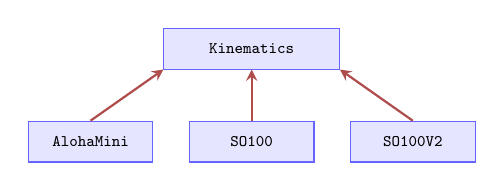
\begin{tikzpicture}[scale=0.65, transform shape]
        % Base interface
        \node[class, text width=3.2cm] (base) at (0,0) {\textbf{Kinematics}};

        % Implementations
        \node[class, text width=2.2cm, below left=1cm and 0.2cm of base] (aloha) {AlohaMini};
        \node[class, text width=2.2cm, below=1cm of base] (so100) {SO100};
        \node[class, text width=2.2cm, below right=1cm and 0.2cm of base] (so100v2) {SO100V2};

        % Arrows
        \draw[arrow] (aloha.north) -- (base.south west);
        \draw[arrow] (so100.north) -- (base.south);
        \draw[arrow] (so100v2.north) -- (base.south east);
    \end{tikzpicture}
\end{column}
\end{columns}
\end{frame}

% ============================================
% SLIDE: 2-Link Planar IK Theory
% ============================================
\begin{frame}{2-Link Planar IK - Theory}
\begin{columns}
\begin{column}{0.5\textwidth}
    \centering
    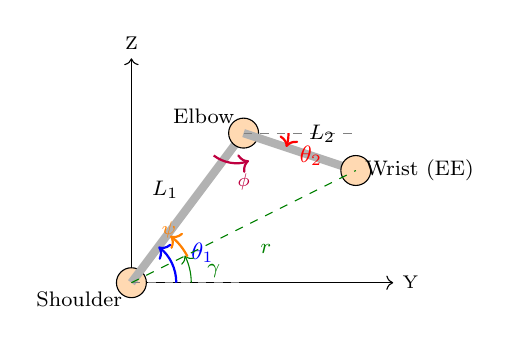
\begin{tikzpicture}[scale=0.95, transform shape]
        % Coordinate axes
        \draw[->] (0,0) -- (3.5,0) node[right] {\scriptsize Y};
        \draw[->] (0,0) -- (0,3) node[above] {\scriptsize Z};

        % Shoulder joint (origin)
        \node[joint] (shoulder) at (0,0) {};
        \node[below left] at (shoulder) {\footnotesize Shoulder};

        % Link 1
        \draw[link] (0,0) -- (1.5,2);
        \node[joint] (elbow) at (1.5,2) {};
        \node[above left] at (elbow) {\footnotesize Elbow};

        % Link 2
        \draw[link] (1.5,2) -- (3,1.5);
        \node[joint] (wrist) at (3,1.5) {};
        \node[right] at (wrist) {\footnotesize Wrist (EE)};

        % theta1: angle of L1 from +Y axis
        \draw[dashed, gray] (0,0) -- (1.5,0);
        \draw[->, blue, thick] (0.6,0) arc (0:53:0.6);
        \node[blue] at (0.95,0.4) {\small $\theta_1$};

        % theta2: exterior angle at elbow
        \draw[dashed, gray] (1.5,2) -- (3,2);
        \draw[->, red, thick] (2.1,2) arc (0:-18:0.6);
        \node[red] at (2.4,1.7) {\small $\theta_2$};

        % phi: interior elbow angle (between L1 and L2)
        \draw[->, purple, thick] (1.1,1.7) arc (233:290:0.5);
        \node[purple, font=\scriptsize] at (1.5,1.35) {$\phi$};

        % Link labels
        \node[above left, font=\footnotesize] at (0.75,1) {$L_1$};
        \node[above right, font=\footnotesize] at (2.25,1.75) {$L_2$};

        % Target line r
        \draw[dashed, green!50!black] (0,0) -- (3,1.5);
        \node[green!50!black, font=\footnotesize] at (1.8,0.45) {$r$};

        % gamma: angle to target from +Y axis
        \draw[->, green!50!black] (0.8,0) arc (0:27:0.8);
        \node[green!50!black, font=\footnotesize] at (1.1,0.15) {$\gamma$};

        % psi: angle between r and L1 (shoulder offset)
        \draw[->, orange, thick] (0.75,0.35) arc (27:53:0.8);
        \node[orange, font=\scriptsize] at (0.5,0.7) {$\psi$};
    \end{tikzpicture}
\end{column}
\begin{column}{0.5\textwidth}
    \textbf{Law of Cosines:}
    \vspace{0.1cm}

    {\small Distance:} $r = \sqrt{y^2 + z^2}$

    \vspace{0.1cm}

    {\small Interior elbow angle ($\phi$):}
    \[\cos\phi = \frac{L_1^2 + L_2^2 - r^2}{2 L_1 L_2}\]

    {\small Shoulder offset ($\psi$):}
    \[\cos\psi = \frac{r^2 + L_1^2 - L_2^2}{2 r L_1}\]

    {\small Joint angles (elbow-up):}
    \[\theta_1 = \gamma - \psi\]
    \[\theta_2 = \theta_1 + (\pi - \phi)\]
\end{column}
\end{columns}
\end{frame}

% ============================================
% SLIDE: AlohaMiniKinematics - Code
% ============================================
\begin{frame}[fragile,shrink=5]{AlohaMiniKinematics - URDF Parameters}
\begin{lstlisting}[basicstyle=\ttfamily\scriptsize]
# URDF Joint Chain (Left Arm):
# left_joint2: xyz=[-0.017, -0.031, 0.054]
# left_joint3: xyz=[0.003, 0.169, 0.043]
# left_joint4: xyz=[0.000, -0.201, 0.005]

class AlohaMiniKinematics:
    def __init__(self):
        # 1.5x extended arm lengths
        self.y3 = 0.16857   # joint3 Y offset
        self.z3 = 0.043244  # joint3 Z offset
        self.y4 = -0.20122  # joint4 Y (NEGATIVE!)
        self.z4 = 0.00544   # joint4 Z offset

        # Link lengths from URDF (Pythagorean)
        self.l1 = sqrt(y3^2 + z3^2)  # ~0.174m
        self.l2 = sqrt(y4^2 + z4^2)  # ~0.201m

        # Geometry angles (measured from +Y axis)
        self.alpha1 = atan2(z3, y3)  # ~14.4 deg
        self.alpha2 = atan2(z4, y4)  # ~178.5 deg
\end{lstlisting}

\vspace{0.15cm}

\begin{block}{Home Position}
At $j_2=0$, $j_3=0$: Wrist at $y=-0.022m$, $z=0.032m$ (Verified: 0.0mm error)
\end{block}
\end{frame}

% ============================================
% SLIDE: AlohaMiniKinematics - FK
% ============================================
\begin{frame}[fragile]{AlohaMiniKinematics - Forward Kinematics}
\begin{lstlisting}
def forward_kinematics(self, j2_deg: float, j3_deg: float) -> Tuple[float, float]:
    """Compute wrist position at joint4."""
    j2 = math.radians(j2_deg)
    j3 = math.radians(j3_deg)

    # Absolute angle of link1 (upper arm) in Y-Z plane
    # When j2=0, link1 points at angle alpha1 from +Y axis
    theta1 = j2 + self.alpha1

    # Absolute angle of link2 (forearm) in Y-Z plane
    # j2 rotates the whole arm, j3 rotates link2 relative to link1
    # alpha2 accounts for the backward-pointing geometry (~178.45 deg)
    theta2 = j2 + j3 + self.alpha2

    # FK: position of j4 relative to j2 in Y-Z plane
    y = self.l1 * math.cos(theta1) + self.l2 * math.cos(theta2)
    z = self.l1 * math.sin(theta1) + self.l2 * math.sin(theta2)

    return y, z
\end{lstlisting}

\begin{block}{Key Insight}
The $\alpha_2 \approx 178.45°$ offset encodes that the forearm points \textbf{backward} in link3's frame. This is why the arm is folded (not extended) at home position.
\end{block}
\end{frame}

% ============================================
% SLIDE: AlohaMiniKinematics - IK
% ============================================
\begin{frame}[fragile]{AlohaMiniKinematics - Inverse Kinematics}
\begin{lstlisting}
def inverse_kinematics(self, y_target: float, z_target: float) -> Tuple[float, float]:
    # Distance from shoulder to target
    r = math.sqrt(y_target**2 + z_target**2)

    # Clamp to workspace
    r_max = self.l1 + self.l2
    r_min = abs(self.l1 - self.l2)
    # ... clamping logic ...

    # Angle to target from +Y axis
    gamma = math.atan2(z_target, y_target)

    # Law of cosines for elbow
    cos_alpha = (r**2 + self.l1**2 - self.l2**2) / (2 * self.l1 * r)
    alpha = math.acos(cos_alpha)

    # Two solutions: theta1 = gamma +/- alpha
    theta1_a = gamma - alpha  # elbow-up
    theta1_b = gamma + alpha  # elbow-down

    # Interior elbow angle
    cos_phi = (self.l1**2 + self.l2**2 - r**2) / (2 * self.l1 * self.l2)
    phi = math.acos(cos_phi)

    # theta2 = theta1 + (pi - phi)  [exterior angle relationship]
    # ... solve and verify with FK ...
\end{lstlisting}
\end{frame}

% ============================================
% SLIDE: SO100Kinematics
% ============================================
\begin{frame}[fragile]{SO100Kinematics - XLeRobot Style}
\begin{columns}
\begin{column}{0.5\textwidth}
\begin{lstlisting}
class SO100Kinematics:
    """XLeRobot-style kinematics."""

    def __init__(self):
        # Link lengths from URDF
        self.l1 = 0.1159  # shoulder-elbow
        self.l2 = 0.1350  # elbow-wrist

        # URDF geometry offsets
        self.theta1_offset = atan2(0.028, 0.11257)
        self.theta2_offset = (
            atan2(0.0052, 0.1349) +
            self.theta1_offset
        )

        # Initial EE position
        self.initial_ee_x = 0.162
        self.initial_ee_y = 0.118
\end{lstlisting}
\end{column}
\begin{column}{0.5\textwidth}
    \textbf{URDF Joint Offsets:}
    \begin{table}
    \centering
    \footnotesize
    \begin{tabular}{lr}
    \toprule
    \textbf{Joint} & \textbf{Offset (XYZ)} \\
    \midrule
    shoulder\_pan & (0, -0.045, 0.017) \\
    shoulder\_lift & (0, 0.103, 0.031) \\
    elbow\_flex & (0, 0.113, 0.028) \\
    wrist\_flex & (0, 0.005, 0.135) \\
    \bottomrule
    \end{tabular}
    \end{table}

    \vspace{0.3cm}

    \textbf{Joint Limits:}
    \begin{itemize}
        \item shoulder\_pan: $\pm 114°$
        \item shoulder\_lift: $-6°$ to $198°$
        \item elbow\_flex: $-11°$ to $180°$
        \item wrist\_flex: $\pm 103°$
    \end{itemize}
\end{column}
\end{columns}
\end{frame}

% ============================================
% SLIDE: SO100Kinematics - IK
% ============================================
\begin{frame}[fragile]{SO100Kinematics - IK with Pitch Compensation}
\begin{lstlisting}
def inverse_kinematics(self, x: float, y: float, pitch: float = 0.0):
    r = math.sqrt(x**2 + y**2)

    # Workspace clamping
    r_max = self.l1 + self.l2
    r_min = abs(self.l1 - self.l2)
    # ... scale if out of bounds ...

    # Law of cosines (NOTE: negative sign is critical!)
    cos_theta2 = -(r**2 - self.l1**2 - self.l2**2) / (2 * self.l1 * self.l2)
    theta2 = math.pi - math.acos(cos_theta2)

    # Shoulder angle using geometric approach
    beta = math.atan2(y, x)
    gamma = math.atan2(self.l2 * sin(theta2), self.l1 + self.l2 * cos(theta2))
    theta1 = beta + gamma

    # Convert to URDF joint angles (add offsets)
    joint2 = theta1 + self.theta1_offset  # shoulder_lift
    joint3 = theta2 + self.theta2_offset  # elbow_flex

    # Wrist flex for pitch compensation
    wrist_flex = joint2 - joint3 + pitch
    return joint2, joint3, wrist_flex
\end{lstlisting}
\end{frame}

% ============================================
% SLIDE: SO100KinematicsV2
% ============================================
\begin{frame}{SO100KinematicsV2 - V2 URDF Structure}
\begin{columns}
\begin{column}{0.5\textwidth}
    \textbf{V2 URDF Differences:}
    \begin{itemize}
        \item shoulder\_pan: 90° X rotation
        \item Transforms coordinates:
        \begin{itemize}
            \item Arm local Y $\rightarrow$ World Z (up)
            \item Arm local Z $\rightarrow$ World -Y (forward)
        \end{itemize}
        \item Uses TCP position directly
    \end{itemize}

    \vspace{0.3cm}

    \textbf{User Coordinates:}
    \begin{itemize}
        \item \code{ee\_x} = forward distance
        \item \code{ee\_y} = height (up)
    \end{itemize}

    \vspace{0.3cm}

    \textbf{TCP at Home:}
    \begin{itemize}
        \item $x = 0.386m$ (forward)
        \item $y = 0.267m$ (up)
    \end{itemize}
\end{column}
\begin{column}{0.5\textwidth}
    \centering
    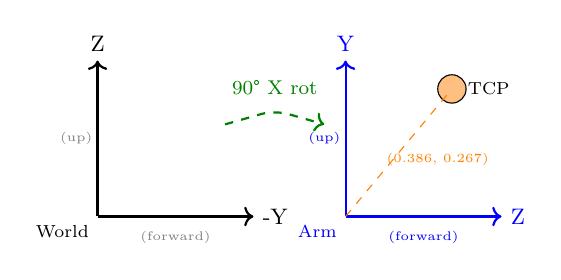
\begin{tikzpicture}[scale=0.9, transform shape]
        % World frame
        \draw[->, thick] (0,0) -- (2.2,0) node[right] {\small -Y};
        \draw[->, thick] (0,0) -- (0,2.2) node[above] {\small Z};
        \node[below left, font=\scriptsize] at (0,0) {World};
        \node[font=\tiny, gray] at (1.1,-0.3) {(forward)};
        \node[font=\tiny, gray] at (-0.3,1.1) {(up)};

        % Arm frame (rotated)
        \draw[->, blue, thick] (3.5,0) -- (5.7,0) node[right] {\small Z};
        \draw[->, blue, thick] (3.5,0) -- (3.5,2.2) node[above] {\small Y};
        \node[below left, blue, font=\scriptsize] at (3.5,0) {Arm};
        \node[font=\tiny, blue] at (4.6,-0.3) {(forward)};
        \node[font=\tiny, blue] at (3.2,1.1) {(up)};

        % Transform arrow with curved path
        \draw[->, thick, green!50!black, dashed, rounded corners=5pt]
            (1.8,1.3) -- (2.5,1.5) -- (3.2,1.3);
        \node[above, green!50!black, font=\footnotesize] at (2.5,1.6) {90° X rot};

        % TCP position with coordinates
        \node[joint, fill=orange!50] at (5,1.8) {};
        \node[right, font=\scriptsize] at (5.1,1.8) {TCP};
        \draw[dashed, orange] (3.5,0) -- (5,1.8);
        \node[font=\tiny, orange] at (4.8,0.8) {(0.386, 0.267)};
    \end{tikzpicture}

    \vspace{0.4cm}

    \begin{block}{Offset Parameters}
    \code{offset\_x = 0.223m}\\
    \code{offset\_y = 0.150m}\\
    (Accounts for base, shoulder, gripper)
    \end{block}
\end{column}
\end{columns}
\end{frame}

% ============================================
% SLIDE: SO100KinematicsV2 - FK/IK
% ============================================
\begin{frame}[fragile]{SO100KinematicsV2 - Consistent FK/IK}
\begin{lstlisting}
def forward_kinematics(self, j2: float, j3: float) -> Tuple[float, float]:
    # Absolute angles in arm's Y-Z plane (from +Y toward +Z)
    theta1 = j2 + self.alpha1  # Link 1 angle
    theta2 = j2 + j3 + self.alpha2  # Link 2 angle

    # Wrist position (Y=up, Z=forward in arm frame)
    wrist_y = self.l1 * cos(theta1) + self.l2 * cos(theta2)
    wrist_z = self.l1 * sin(theta1) + self.l2 * sin(theta2)

    # Transform to user coordinates
    ee_x = wrist_z + self.offset_x  # forward
    ee_y = wrist_y + self.offset_y  # up
    return ee_x, ee_y

def inverse_kinematics(self, x: float, y: float, pitch: float = 0.0):
    # Transform TCP to wrist position
    wrist_z = x - self.offset_x
    wrist_y = y - self.offset_y
    # ... law of cosines solution (same as AlohaMiniKinematics) ...
    # Convert: j2 = theta1 - alpha1, j3 = theta2 - theta1 + alpha1 - alpha2
\end{lstlisting}
\end{frame}

% ============================================
% SLIDE: Verification Results
% ============================================
\begin{frame}[shrink=5]{Kinematics Verification Results}
\begin{columns}
\begin{column}{0.5\textwidth}
    \textbf{AlohaMiniKinematics:}
    \begin{table}
    \centering
    \footnotesize
    \begin{tabular}{lr}
    \toprule
    \textbf{Test} & \textbf{Result} \\
    \midrule
    FK at home & 0.0mm error \\
    IK round-trip & 0.0mm error \\
    Joint tracking & 0.0° error \\
    \bottomrule
    \end{tabular}
    \end{table}

    \vspace{0.2cm}

    \begin{alertblock}{Warning in Code}
    \scriptsize
    ``DO NOT MODIFY THIS IK/FK CODE''\\
    ``Verified working perfectly: 2024-12-31''
    \end{alertblock}
\end{column}
\begin{column}{0.5\textwidth}
    \textbf{SO100KinematicsV2:}
    \begin{table}
    \centering
    \footnotesize
    \begin{tabular}{lr}
    \toprule
    \textbf{Test} & \textbf{Result} \\
    \midrule
    FK at home & 0.0mm error \\
    IK at home & $\sim$0° joint error \\
    Position round-trip & $<$1mm error \\
    \bottomrule
    \end{tabular}
    \end{table}

    \vspace{0.2cm}

    \textbf{Test Cases:}
    \begin{itemize}
        \item Joint angles: 10 test cases
        \item Position targets: 8 test cases
        \item All pass with $<$1mm error
    \end{itemize}
\end{column}
\end{columns}

\vspace{0.2cm}

\begin{block}{Key Insight}
\small Mathematical consistency between FK and IK is critical. Both must use the same geometry angles ($\alpha_1$, $\alpha_2$) and coordinate transformations.
\end{block}
\end{frame}

% ============================================
% SLIDE: Workspace Visualization
% ============================================
\begin{frame}{Workspace Visualization}
\begin{columns}
\begin{column}{0.55\textwidth}
    \centering
    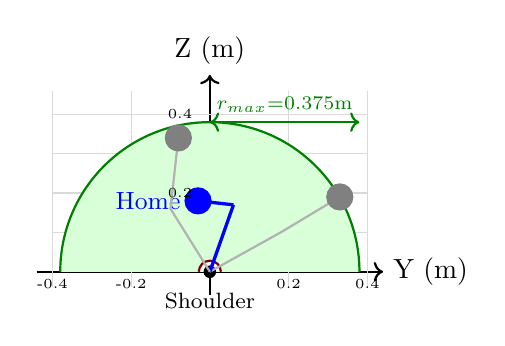
\begin{tikzpicture}[scale=1.0, transform shape]
        % Coordinate axes
        \draw[->, thick] (-2.2,0) -- (2.2,0) node[right] {Y (m)};
        \draw[->, thick] (0,-0.3) -- (0,2.5) node[above] {Z (m)};

        % Grid lines (light)
        \foreach \x in {-2,-1,1,2} {
            \draw[gray!30, thin] (\x,-0.2) -- (\x,2.3);
        }
        \foreach \y in {0.5,1,1.5,2} {
            \draw[gray!30, thin] (-2,\y) -- (2,\y);
        }

        % Workspace annulus (upper half only - arm operates in Y-Z plane)
        \fill[green!15] (0,0) -- (1.9,0) arc (0:180:1.9) -- cycle;
        \fill[white] (0,0) -- (0.14,0) arc (0:180:0.14) -- cycle;

        % Boundary circles
        \draw[green!50!black, thick] (0,0) ++(0:1.9) arc (0:180:1.9);
        \draw[red!50!black, thick] (0,0) ++(0:0.14) arc (0:180:0.14);

        % Shoulder joint
        \fill[black] (0,0) circle (0.08);
        \node[below=0.15cm] at (0,0) {\footnotesize Shoulder};

        % Sample arm configurations
        % Extended pose (right side)
        \draw[thick, gray!60] (0,0) -- (0.9,0.5) -- (1.65,0.95);
        \node[joint, gray, minimum size=0.12cm] at (1.65,0.95) {};

        % Folded pose (home) - moved slightly left
        \draw[very thick, blue] (0,0) -- (0.3,0.85);
        \draw[very thick, blue] (0.3,0.85) -- (-0.15,0.9);
        \node[joint, blue, minimum size=0.15cm] at (-0.15,0.9) {};
        \node[blue, font=\small, left] at (-0.25,0.9) {Home};

        % Upward pose (left side)
        \draw[thick, gray!60] (0,0) -- (-0.5,0.8) -- (-0.4,1.7);
        \node[joint, gray, minimum size=0.12cm] at (-0.4,1.7) {};

        % r_max indicator - horizontal line at top
        \draw[<->, green!50!black, thick] (0,1.9) -- (1.9,1.9);
        \node[green!50!black, font=\scriptsize, above] at (0.95,1.9) {$r_{max}$=0.375m};

        % Scale markers
        \node[font=\tiny] at (-2,-0.15) {-0.4};
        \node[font=\tiny] at (-1,-0.15) {-0.2};
        \node[font=\tiny] at (1,-0.15) {0.2};
        \node[font=\tiny] at (2,-0.15) {0.4};
        \node[font=\tiny, left] at (-0.1,1) {0.2};
        \node[font=\tiny, left] at (-0.1,2) {0.4};
    \end{tikzpicture}
\end{column}
\begin{column}{0.45\textwidth}
    \textbf{Workspace Definition:}
    \begin{itemize}
        \item Shoulder at origin (0, 0)
        \item Arm operates in Y-Z plane
        \item Green area = reachable zone
    \end{itemize}

    \vspace{0.3cm}

    \textbf{Boundaries:}
    \begin{itemize}
        \item $r_{max} = L_1 + L_2 = 0.375$m
        \item $r_{min} = |L_1 - L_2| = 0.027$m
    \end{itemize}

    \vspace{0.3cm}

    \textbf{Arm Poses:}
    \begin{itemize}
        \item \textcolor{blue}{Blue}: Home (folded)
        \item \textcolor{gray}{Gray}: Sample configs
    \end{itemize}
\end{column}
\end{columns}
\end{frame}

% ============================================
% SLIDE: Workspace Parameters
% ============================================
\begin{frame}{Workspace Parameters}
\begin{columns}
\begin{column}{0.5\textwidth}
    \textbf{AlohaMiniKinematics:}
    \begin{table}
    \centering
    \footnotesize
    \begin{tabular}{lr}
    \toprule
    \textbf{Parameter} & \textbf{Value} \\
    \midrule
    $L_1$ (upper arm) & 0.174m \\
    $L_2$ (forearm) & 0.201m \\
    $r_{min}$ & 0.027m \\
    $r_{max}$ & 0.375m \\
    \bottomrule
    \end{tabular}
    \end{table}
\end{column}
\begin{column}{0.5\textwidth}
    \textbf{SO100Kinematics:}
    \begin{table}
    \centering
    \footnotesize
    \begin{tabular}{lr}
    \toprule
    \textbf{Parameter} & \textbf{Value} \\
    \midrule
    $L_1$ (upper arm) & 0.116m \\
    $L_2$ (forearm) & 0.135m \\
    $r_{min}$ & 0.019m \\
    $r_{max}$ & 0.251m \\
    \bottomrule
    \end{tabular}
    \end{table}
\end{column}
\end{columns}

\vspace{0.5cm}

\begin{block}{Workspace Clamping}
IK clamps targets to $[r_{min} \times 1.01, r_{max} \times 0.99]$ to avoid singularities at workspace boundaries.
\end{block}
\end{frame}

% ============================================
% SLIDE: Wrist Flex Compensation
% ============================================
\begin{frame}{Wrist Flex / Pitch Compensation}
\begin{columns}
\begin{column}{0.5\textwidth}
    \centering
    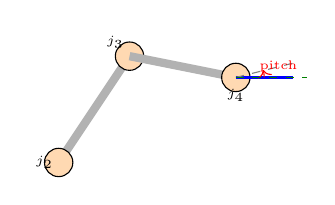
\begin{tikzpicture}[scale=0.9, transform shape]
        % Arm links
        \draw[link] (0,0) -- (1,1.5);
        \node[joint] at (0,0) {};
        \node[joint] at (1,1.5) {};

        \draw[link] (1,1.5) -- (2.5,1.2);
        \node[joint] at (2.5,1.2) {};

        % Gripper
        \draw[thick, blue] (2.5,1.2) -- (3.3,1.2);

        % Pitch angle indicator
        \draw[dashed, gray] (2.5,1.2) -- (3.3,1.4);
        \draw[->, red] (2.9,1.2) arc (0:15:0.4);
        \node[red, font=\tiny] at (3.1,1.35) {pitch};

        % Level line
        \draw[dashed, green!50!black] (2.5,1.2) -- (3.5,1.2);

        % Joint labels
        \node[font=\tiny] at (-0.2,0) {$j_2$};
        \node[font=\tiny] at (0.8,1.7) {$j_3$};
        \node[font=\tiny] at (2.5,0.95) {$j_4$};
    \end{tikzpicture}

    \vspace{0.3cm}

    \textbf{Pitch Formula:}
    \[pitch_{EE} = j_2 + j_3 + j_4\]

    For level gripper ($pitch=0$):
    \[j_4 = -j_2 - j_3\]
\end{column}
\begin{column}{0.5\textwidth}
    \textbf{Implementation Variants:}

    \vspace{0.2cm}

    \textbf{AlohaMiniKinematics:}
    \begin{itemize}
        \item \code{j4 = pitch - j2 - j3}
    \end{itemize}

    \vspace{0.2cm}

    \textbf{SO100Kinematics:}
    \begin{itemize}
        \item \code{wrist = j2 - j3 + pitch}
    \end{itemize}

    \vspace{0.2cm}

    \textbf{SO100KinematicsV2:}
    \begin{itemize}
        \item \code{wrist = pitch - (j2 + j3)}
    \end{itemize}

    \vspace{0.3cm}

    \begin{block}{Key Insight}
    Setting \code{pitch=0} keeps gripper level regardless of arm pose.
    \end{block}
\end{column}
\end{columns}
\end{frame}

% ============================================
% SLIDE: Module Summary
% ============================================
\begin{frame}{Kinematics Module Summary}
\begin{columns}
\begin{column}{0.55\textwidth}
    \textbf{Key Design Decisions:}
    \begin{enumerate}
        \item 2-link planar IK (Y-Z plane)
        \item Law of cosines solution
        \item URDF geometry offsets
        \item Workspace clamping
        \item Pitch compensation
    \end{enumerate}

    \vspace{0.2cm}

    \textbf{Important Constants:}
    \begin{itemize}
        \item Link lengths from URDF
        \item Geometry angles ($\alpha_1$, $\alpha_2$)
        \item TCP offsets (V2 only)
    \end{itemize}
\end{column}
\begin{column}{0.45\textwidth}
    \centering
    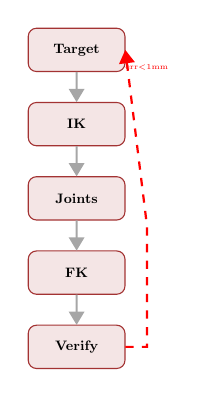
\begin{tikzpicture}[scale=0.55, transform shape, node distance=0.7cm]
        % Flow diagram
        \node[module, text width=2cm] (target) {Target};
        \node[module, text width=2cm, below=of target] (ik) {IK};
        \node[module, text width=2cm, below=of ik] (joints) {Joints};
        \node[module, text width=2cm, below=of joints] (fk) {FK};
        \node[module, text width=2cm, below=of fk] (verify) {Verify};

        % Arrows
        \draw[flow] (target) -- (ik);
        \draw[flow] (ik) -- (joints);
        \draw[flow] (joints) -- (fk);
        \draw[flow] (fk) -- (verify);

        % Verification loop
        \draw[flow, dashed, red] (verify.east) -- ++(0.5,0) -- ++(0,2.8) -- (target.east);
        \node[right, font=\tiny, red] at (1.0,-0.4) {err$<$1mm};
    \end{tikzpicture}

    \begin{alertblock}{Critical}
    \scriptsize FK and IK must be mathematically consistent!
    \end{alertblock}
\end{column}
\end{columns}
\end{frame}



% ============================================
% SECTION 5: LEROBOT (PHYSICAL ROBOT)
% ============================================
% 05_lerobot.tex - Physical Robot Module
% AlohaMini Codebase Documentation

\section{LeRobot Module (Physical Robot)}

% ============================================
% SLIDE: Module Overview
% ============================================
\begin{frame}{software/ Module Overview}
\begin{columns}
\begin{column}{0.4\textwidth}
    \textbf{Purpose:} Physical robot control via LeRobot framework

    \vspace{0.2cm}

    \textbf{Key Files:}
    \begin{itemize}
        \item \filepath{lekiwi.py} (642 lines)
        \item \filepath{config\_lekiwi.py} (114 lines)
        \item \filepath{lift\_axis.py} (217 lines)
    \end{itemize}

    \vspace{0.2cm}

    \textbf{Dependencies:}
    \begin{itemize}
        \item LeRobot framework
        \item Feetech motors (STS3215)
        \item OpenCV cameras
    \end{itemize}
\end{column}
\begin{column}{0.6\textwidth}
    \centering
    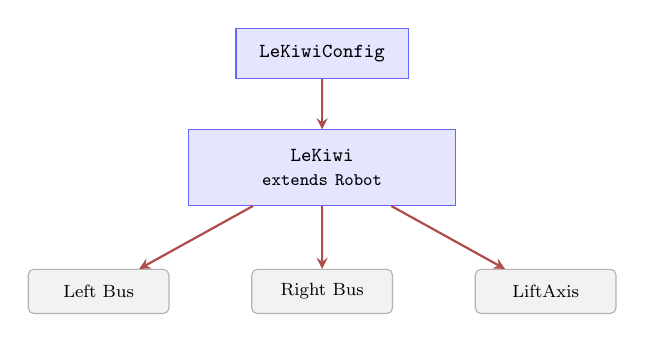
\begin{tikzpicture}[scale=0.8, transform shape]
        % Main robot class
        \node[class, text width=4cm, minimum height=1.2cm] (lekiwi) at (0,0) {
            \textbf{LeKiwi}\\
            \footnotesize extends Robot
        };

        % Components
        \node[submodule, text width=2cm, below left=1cm and 0.3cm of lekiwi] (left) {
            Left Bus
        };
        \node[submodule, text width=2cm, below=1cm of lekiwi] (right) {
            Right Bus
        };
        \node[submodule, text width=2cm, below right=1cm and 0.3cm of lekiwi] (lift) {
            LiftAxis
        };

        % Config
        \node[class, text width=2.5cm, above=0.8cm of lekiwi] (config) {
            LeKiwiConfig
        };

        % Arrows
        \draw[arrow] (config) -- (lekiwi);
        \draw[arrow] (lekiwi) -- (left);
        \draw[arrow] (lekiwi) -- (right);
        \draw[arrow] (lekiwi) -- (lift);
    \end{tikzpicture}
\end{column}
\end{columns}
\end{frame}

% ============================================
% SLIDE: Hardware Architecture
% ============================================
\begin{frame}{AlohaMini Hardware Architecture}
\centering
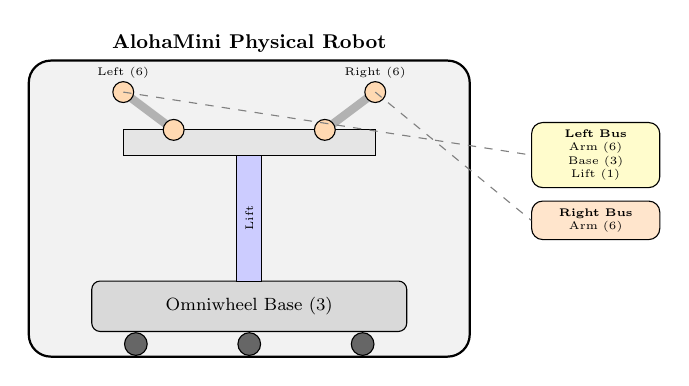
\begin{tikzpicture}[scale=0.8, transform shape]
    % Robot outline
    \draw[rounded corners=8pt, thick, fill=gray!10] (-3.5,-1.2) rectangle (3.5,3.5);
    \node[above, font=\bfseries\small] at (0,3.5) {AlohaMini Physical Robot};

    % Mobile base
    \draw[fill=gray!30, rounded corners=3pt] (-2.5,-0.8) rectangle (2.5,0);
    \node[font=\footnotesize] at (0,-0.4) {Omniwheel Base (3)};

    % Wheels
    \draw[fill=black!60] (-1.8,-1) circle (0.18);
    \draw[fill=black!60] (1.8,-1) circle (0.18);
    \draw[fill=black!60] (0,-1) circle (0.18);

    % Lift column
    \draw[fill=blue!20] (-0.2,0) rectangle (0.2,2);
    \node[rotate=90, font=\tiny] at (0,1) {Lift};

    % Arm platform
    \draw[fill=gray!20] (-2,2) rectangle (2,2.4);

    % Left arm
    \draw[link] (-1.2,2.4) -- (-2,3);
    \node[joint, minimum size=0.25cm] at (-1.2,2.4) {};
    \node[joint, minimum size=0.25cm] at (-2,3) {};
    \node[font=\tiny] at (-2,3.3) {Left (6)};

    % Right arm
    \draw[link] (1.2,2.4) -- (2,3);
    \node[joint, minimum size=0.25cm] at (1.2,2.4) {};
    \node[joint, minimum size=0.25cm] at (2,3) {};
    \node[font=\tiny] at (2,3.3) {Right (6)};

    % Bus connections (right side)
    \node[draw, rounded corners, fill=yellow!20, text width=1.8cm, font=\tiny, align=center] (leftbus) at (5.5,2) {
        \textbf{Left Bus}\\
        Arm (6)\\
        Base (3)\\
        Lift (1)
    };
    \node[draw, rounded corners, fill=orange!20, text width=1.8cm, font=\tiny, align=center, below=0.2cm of leftbus] (rightbus) {
        \textbf{Right Bus}\\
        Arm (6)
    };

    % Connection lines
    \draw[dashed, gray, thin] (2,3) -- (rightbus.west);
    \draw[dashed, gray, thin] (-2,3) -- (leftbus.west);
\end{tikzpicture}
\end{frame}

% ============================================
% SLIDE: Motor Configuration
% ============================================
\begin{frame}[fragile]{LeKiwi - Motor Configuration}
\begin{lstlisting}[basicstyle=\ttfamily\scriptsize]
self.left_bus = FeetechMotorsBus(
    port=self.config.left_port,
    motors={
        # Left arm joints (6 DOF)
        "arm_left_shoulder_pan": Motor(1, "sts3215", norm_mode),
        "arm_left_shoulder_lift": Motor(2, "sts3215", norm_mode),
        "arm_left_elbow_flex": Motor(3, "sts3215", norm_mode),
        "arm_left_wrist_flex": Motor(4, "sts3215", norm_mode),
        "arm_left_wrist_roll": Motor(5, "sts3215", norm_mode),
        "arm_left_gripper": Motor(6, "sts3215", RANGE_0_100),
        # Mobile base (3 wheels)
        "base_left_wheel": Motor(8, "sts3215", RANGE_M100_100),
        "base_back_wheel": Motor(9, "sts3215", RANGE_M100_100),
        "base_right_wheel": Motor(10, "sts3215", RANGE_M100_100),
        # Lift mechanism
        "lift_axis": Motor(11, "sts3215", DEGREES),
    },
)
\end{lstlisting}
\end{frame}

% ============================================
% SLIDE: State Features
% ============================================
\begin{frame}{LeKiwi - State/Action Features}
\begin{columns}
\begin{column}{0.5\textwidth}
    \textbf{State Features (16 DOF):}
    \begin{itemize}
        \item \code{arm\_left\_*.pos} (6)
        \item \code{arm\_right\_*.pos} (6)
        \item \code{x.vel, y.vel, theta.vel} (3)
        \item \code{lift\_axis.height\_mm} (1)
    \end{itemize}

    \vspace{0.3cm}

    \textbf{Camera Features (5):}
    \begin{itemize}
        \item head\_top, head\_back, head\_front
        \item wrist\_left, wrist\_right
        \item Resolution: 640$\times$480
    \end{itemize}
\end{column}
\begin{column}{0.5\textwidth}
    \begin{table}
    \centering
    \footnotesize
    \begin{tabular}{lr}
    \toprule
    \textbf{Component} & \textbf{DOF} \\
    \midrule
    Left Arm & 6 \\
    Right Arm & 6 \\
    Base Velocity & 3 \\
    Lift Height & 1 \\
    \midrule
    \textbf{Total} & \textbf{16} \\
    \bottomrule
    \end{tabular}
    \end{table}

    \vspace{0.3cm}

    \begin{block}{Action = State}
    Action features mirror state features for teleoperation recording.
    \end{block}
\end{column}
\end{columns}
\end{frame}

% ============================================
% SLIDE: Omniwheel Kinematics
% ============================================
\begin{frame}{Omniwheel Base Kinematics}
\begin{columns}
\begin{column}{0.45\textwidth}
    \centering
    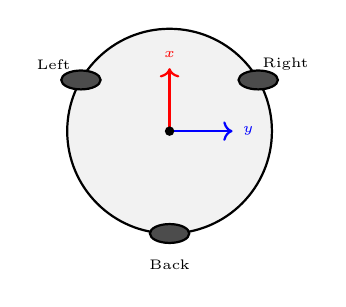
\begin{tikzpicture}[scale=1.0, transform shape]
        % Robot base circle
        \draw[thick, fill=gray!10] (0,0) circle (1.3);

        % Wheel positions
        \foreach \angle in {150, 270, 30} {
            \draw[fill=black!70, thick] (\angle:1.3) ellipse (0.25 and 0.12);
        }

        % Wheel labels
        \node[font=\tiny] at (150:1.7) {Left};
        \node[font=\tiny] at (270:1.7) {Back};
        \node[font=\tiny] at (30:1.7) {Right};

        % Coordinate frame
        \draw[->, thick, red] (0,0) -- (0,0.8) node[above, font=\tiny] {$x$};
        \draw[->, thick, blue] (0,0) -- (0.8,0) node[right, font=\tiny] {$y$};

        % Center
        \fill (0,0) circle (0.06);
    \end{tikzpicture}
\end{column}
\begin{column}{0.55\textwidth}
    \textbf{Inverse Kinematics:}

    Wheel angles: $\phi_i = [150°, 270°, 30°]$

    \vspace{0.2cm}

    Kinematic matrix:
    \[M = \begin{bmatrix}
        \cos\phi_1 & \sin\phi_1 & R \\
        \cos\phi_2 & \sin\phi_2 & R \\
        \cos\phi_3 & \sin\phi_3 & R
    \end{bmatrix}\]

    Body to wheel: $\vec{\omega} = \frac{M \cdot \vec{v}}{r}$

    \vspace{0.2cm}

    \textbf{Parameters:}
    \begin{itemize}
        \item $r_{wheel} = 0.05m$
        \item $R_{base} = 0.125m$
    \end{itemize}
\end{column}
\end{columns}
\end{frame}

% ============================================
% SLIDE: Body to Wheel Conversion
% ============================================
\begin{frame}[fragile]{Body to Wheel Conversion}
\begin{lstlisting}[basicstyle=\ttfamily\scriptsize]
def _body_to_wheel_raw(self, x, y, theta, wheel_radius=0.05,
                       base_radius=0.125, max_raw=3000):
    """Convert body velocities (x, y, theta) to wheel raw commands."""
    theta_rad = theta * (np.pi / 180.0)
    velocity_vector = np.array([-x, -y, theta_rad])

    # Wheel mounting angles with -90 deg offset
    angles = np.radians(np.array([240, 0, 120]) - 90)
    m = np.array([[np.cos(a), np.sin(a), base_radius] for a in angles])

    # Compute wheel speeds
    wheel_linear_speeds = m.dot(velocity_vector)
    wheel_angular_speeds = wheel_linear_speeds / wheel_radius
    wheel_degps = wheel_angular_speeds * (180.0 / np.pi)

    # Scale if exceeds max_raw ...
    wheel_raw = [self._degps_to_raw(deg) for deg in wheel_degps]
    return {"base_left_wheel": wheel_raw[0], ...}
\end{lstlisting}
\end{frame}

% ============================================
% SLIDE: LiftAxis Config
% ============================================
\begin{frame}[fragile]{LiftAxis - Configuration}
\begin{columns}
\begin{column}{0.55\textwidth}
\begin{lstlisting}[basicstyle=\ttfamily\scriptsize]
@dataclass
class LiftAxisConfig:
    enabled: bool = True
    name: str = "lift_axis"
    motor_id: int = 11

    # Lead screw parameters
    lead_mm_per_rev: float = 84
    soft_min_mm: float = 0.0
    soft_max_mm: float = 600

    # Homing parameters
    home_down_speed: int = 1300
    home_stall_current_ma: int = 150

    # Velocity control
    kp_vel: float = 300
    v_max: int = 1300
    dir_sign: int = -1
\end{lstlisting}
\end{column}
\begin{column}{0.45\textwidth}
    \textbf{Key Features:}
    \begin{itemize}
        \item Multi-turn tracking
        \item Velocity closed-loop
        \item Automatic homing
        \item Soft limits
    \end{itemize}

    \vspace{0.3cm}

    \textbf{Position Calc:}
    \begin{align*}
        h_{mm} &= (\theta - \theta_0) \\
               &\quad \times \frac{lead}{360°}
    \end{align*}
\end{column}
\end{columns}
\end{frame}

% ============================================
% SLIDE: LiftAxis Homing
% ============================================
\begin{frame}{LiftAxis - Homing Procedure}
\begin{columns}
\begin{column}{0.5\textwidth}
    \textbf{Homing Algorithm:}
    \begin{enumerate}
        \item Drive down at \code{home\_down\_speed}
        \item Monitor current (6.5x scale)
        \item Detect stall (\textgreater 1500mA)
        \item Set current position as z=0
    \end{enumerate}
\end{column}
\begin{column}{0.5\textwidth}
    \textbf{Parameters:}
    \begin{itemize}
        \item Timeout: 30 seconds
        \item Poll rate: 50ms
        \item Stall threshold: 2 consecutive
        \item Current limit: 1500 mA
    \end{itemize}
\end{column}
\end{columns}
\end{frame}

% ============================================
% SLIDE: Observation Flow
% ============================================
\begin{frame}{LeKiwi - Observation \& Action Flow}
\centering
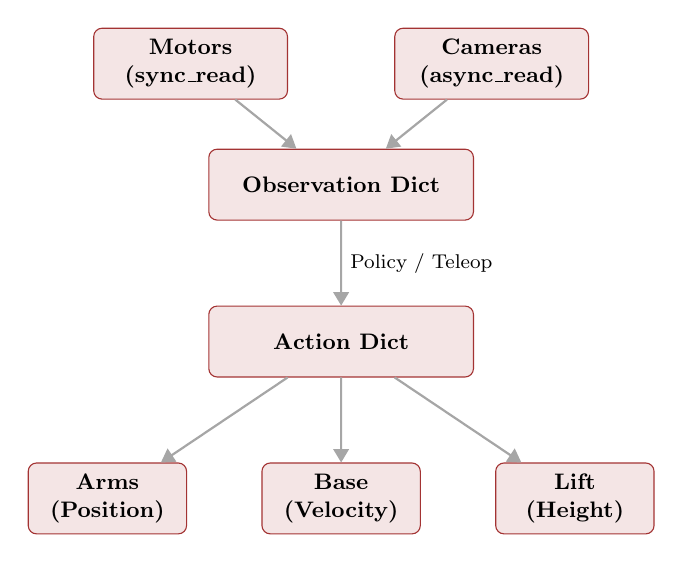
\begin{tikzpicture}[scale=0.9, transform shape, node distance=1.2cm]
    % Observation flow
    \node[module, text width=2.5cm] (motors) at (0,0) {Motors\\(sync\_read)};
    \node[module, text width=2.5cm, right=1.5cm of motors] (cameras) {Cameras\\(async\_read)};
    \node[module, text width=3.5cm, below=1.2cm of $(motors)!0.5!(cameras)$] (obs) {Observation Dict};

    % Action flow
    \node[module, text width=3.5cm, below=of obs] (action) {Action Dict};
    \node[module, text width=2cm, below left=1.2cm and 0.3cm of action] (arm) {Arms\\(Position)};
    \node[module, text width=2cm, below=1.2cm of action] (base) {Base\\(Velocity)};
    \node[module, text width=2cm, below right=1.2cm and 0.3cm of action] (lift) {Lift\\(Height)};

    % Arrows
    \draw[flow] (motors) -- (obs);
    \draw[flow] (cameras) -- (obs);
    \draw[flow] (obs) -- node[right, font=\footnotesize] {Policy / Teleop} (action);
    \draw[flow] (action) -- (arm);
    \draw[flow] (action) -- (base);
    \draw[flow] (action) -- (lift);
\end{tikzpicture}
\end{frame}

% ============================================
% SLIDE: Safety Features
% ============================================
\begin{frame}{LeKiwi - Safety Features}
\begin{columns}
\begin{column}{0.5\textwidth}
    \textbf{1. Overcurrent Protection}
    \begin{itemize}
        \item Default limit: 2000 mA
        \item Scale factor: 6.5 (STS3215)
        \item Emergency stop on exceed
        \item Auto-disconnect
    \end{itemize}

    \vspace{0.3cm}

    \textbf{2. Position Safety}
    \begin{itemize}
        \item \code{max\_relative\_target}
        \item Caps relative motion magnitude
        \item Prevents sudden jumps
    \end{itemize}
\end{column}
\begin{column}{0.5\textwidth}
    \textbf{3. Lift Soft Limits}
    \begin{itemize}
        \item \code{soft\_min\_mm = 0}
        \item \code{soft\_max\_mm = 600}
        \item Velocity blocked at limits
    \end{itemize}

    \vspace{0.3cm}

    \textbf{4. Watchdog (Client Mode)}
    \begin{itemize}
        \item Timeout: 1500 ms
        \item Stops robot if no command
        \item Network disconnection safety
    \end{itemize}
\end{column}
\end{columns}
\end{frame}

% ============================================
% SLIDE: Calibration Process
% ============================================
\begin{frame}{Calibration Process}
\begin{columns}
\begin{column}{0.5\textwidth}
    \textbf{Dual-Bus Calibration:}
    \begin{enumerate}
        \item Disable torque on arm motors
        \item Move LEFT arm to middle
        \item Record half-turn homing offset
        \item Move through full ROM
        \item Record min/max positions
        \item Repeat for RIGHT arm
        \item Merge and save calibration
    \end{enumerate}
\end{column}
\begin{column}{0.5\textwidth}
    \centering
    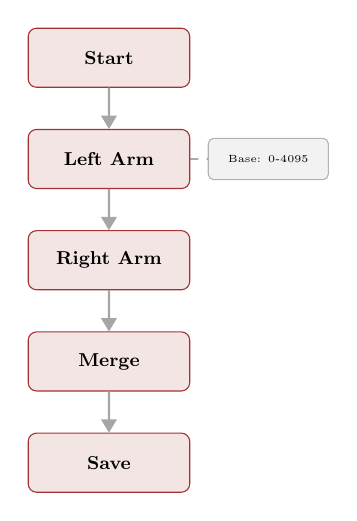
\begin{tikzpicture}[scale=0.75, transform shape, node distance=0.7cm]
        \node[module, text width=2.5cm] (start) {Start};
        \node[module, text width=2.5cm, below=of start] (left) {Left Arm};
        \node[module, text width=2.5cm, below=of left] (right) {Right Arm};
        \node[module, text width=2.5cm, below=of right] (merge) {Merge};
        \node[module, text width=2.5cm, below=of merge] (save) {Save};

        \draw[flow] (start) -- (left);
        \draw[flow] (left) -- (right);
        \draw[flow] (right) -- (merge);
        \draw[flow] (merge) -- (save);

        \node[submodule, text width=1.8cm, right=0.3cm of left, font=\tiny] (base) {Base: 0-4095};
        \draw[dashed, gray] (left) -- (base);
    \end{tikzpicture}
\end{column}
\end{columns}
\end{frame}

% ============================================
% SLIDE: LeKiwiConfig
% ============================================
\begin{frame}[fragile]{LeKiwiConfig}
\begin{lstlisting}[basicstyle=\ttfamily\scriptsize]
@RobotConfig.register_subclass("lekiwi")
@dataclass
class LeKiwiConfig(RobotConfig):
    left_port: str = "/dev/am_arm_follower_left"
    right_port: str = "/dev/am_arm_follower_right"
    disable_torque_on_disconnect: bool = True
    max_relative_target: int | None = None
    cameras: dict[str, CameraConfig] = field(default_factory=...)
    use_degrees: bool = False
\end{lstlisting}

\vspace{0.3cm}

\textbf{Camera Device Paths:}
\begin{itemize}
    \item \code{/dev/am\_camera\_head\_top}
    \item \code{/dev/am\_camera\_head\_back}, \code{head\_front}
    \item \code{/dev/am\_camera\_wrist\_left}, \code{wrist\_right}
\end{itemize}
\end{frame}

% ============================================
% SLIDE: Module Summary
% ============================================
\begin{frame}{LeRobot Module Summary}
\begin{columns}
\begin{column}{0.5\textwidth}
    \textbf{Key Classes:}
    \begin{itemize}
        \item \code{LeKiwi} - Robot interface
        \item \code{LeKiwiConfig} - Configuration
        \item \code{LiftAxis} - Z-axis controller
    \end{itemize}

    \vspace{0.3cm}

    \textbf{Hardware:}
    \begin{itemize}
        \item Feetech STS3215 servos
        \item FeetechMotorsBus
        \item 5 OpenCV cameras
    \end{itemize}
\end{column}
\begin{column}{0.5\textwidth}
    \textbf{Control Modes:}
    \begin{table}
    \centering
    \footnotesize
    \begin{tabular}{ll}
    \toprule
    \textbf{Component} & \textbf{Mode} \\
    \midrule
    Arms & Position \\
    Base wheels & Velocity \\
    Lift axis & Velocity \\
    \bottomrule
    \end{tabular}
    \end{table}

    \vspace{0.3cm}

    \textbf{Control Loop:} 30-50 Hz
\end{column}
\end{columns}
\end{frame}



% ============================================
% SECTION 6: ROS SIMULATION
% ============================================
% 06_simulation.tex - ROS Simulation Module
% AlohaMini Codebase Documentation

\section{ROS Simulation}

% ============================================
% SLIDE: Module Overview
% ============================================
\begin{frame}{simulation/ Module Overview}
\begin{columns}
\begin{column}{0.4\textwidth}
    \textbf{Purpose:} ROS visualization \& physics

    \vspace{0.2cm}

    \textbf{Structure:}
    \begin{itemize}
        \item \filepath{src/Aloha/} - ROS package
        \item \filepath{urdf/} - Robot model
        \item \filepath{meshes/} - STL files
        \item \filepath{launch/} - Launch files
    \end{itemize}

    \vspace{0.2cm}

    \textbf{Support:}
    \begin{itemize}
        \item ROS1 Noetic / ROS2 Humble
        \item RViz / Gazebo
    \end{itemize}
\end{column}
\begin{column}{0.6\textwidth}
    \centering
    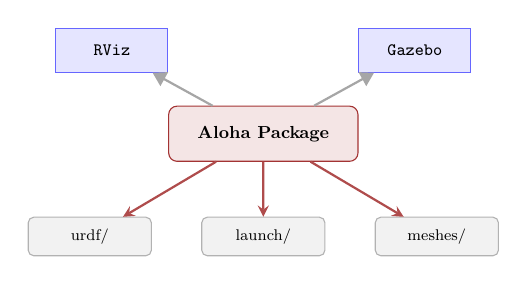
\begin{tikzpicture}[scale=0.7, transform shape]
        % Package structure
        \node[module, text width=3.2cm] (pkg) at (0,0) {\textbf{Aloha Package}};

        % Components
        \node[submodule, text width=2cm, below left=1cm and 0.3cm of pkg] (urdf) {urdf/};
        \node[submodule, text width=2cm, below=1cm of pkg] (launch) {launch/};
        \node[submodule, text width=2cm, below right=1cm and 0.3cm of pkg] (meshes) {meshes/};

        % Arrows
        \draw[arrow] (pkg) -- (urdf);
        \draw[arrow] (pkg) -- (launch);
        \draw[arrow] (pkg) -- (meshes);

        % Tools
        \node[class, text width=1.8cm, above left=0.6cm and 0cm of pkg] (rviz) {RViz};
        \node[class, text width=1.8cm, above right=0.6cm and 0cm of pkg] (gazebo) {Gazebo};

        \draw[flow] (pkg) -- (rviz);
        \draw[flow] (pkg) -- (gazebo);
    \end{tikzpicture}
\end{column}
\end{columns}
\end{frame}

% ============================================
% SLIDE: URDF Structure
% ============================================
\begin{frame}{URDF Robot Model}
\begin{columns}
\begin{column}{0.5\textwidth}
    \textbf{Link/Joint Structure:}
    \begin{itemize}
        \item \code{base\_link} - Robot base
        \item \code{wheel1-3} - Omniwheels
        \item \code{vertical\_move} - Lift
        \item \code{left\_joint1..6} - Left arm
        \item \code{right\_joint1..6} - Right arm
    \end{itemize}

    \vspace{0.2cm}

    \textbf{Total:} 17 joints (3 + 1 + 6 + 6 + gripper)
\end{column}
\begin{column}{0.5\textwidth}
    \centering
    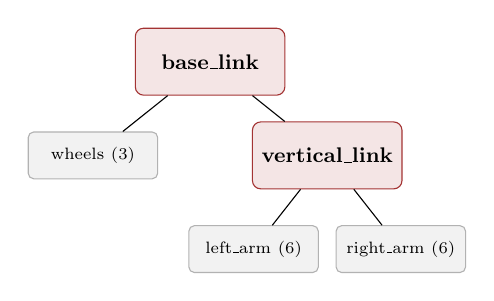
\begin{tikzpicture}[scale=0.85, transform shape, level distance=1.4cm,
        level 1/.style={sibling distance=3.5cm},
        level 2/.style={sibling distance=2.2cm}]
        \node[module, text width=2cm] {base\_link}
            child {node[submodule, text width=1.7cm] {\scriptsize wheels (3)}}
            child {node[module, text width=2cm] {vertical\_link}
                child {node[submodule, text width=1.7cm] {\scriptsize left\_arm (6)}}
                child {node[submodule, text width=1.7cm] {\scriptsize right\_arm (6)}}
            };
    \end{tikzpicture}
\end{column}
\end{columns}
\end{frame}

% ============================================
% SLIDE: Joint Configuration
% ============================================
\begin{frame}[fragile]{Joint Names Configuration}
\begin{lstlisting}[basicstyle=\ttfamily\scriptsize]
# config/joint_names_Aloha.yaml
controller_joint_names: [
    '',              # Empty (index 0)
    'wheel1', 'wheel2', 'wheel3',         # Wheels
    'vertical_move',                       # Lift
    'left_joint1', ..., 'left_joint6',    # Left arm
    'right_joint1', ..., 'right_joint6',  # Right arm
]
\end{lstlisting}

\vspace{0.3cm}

\textbf{Joint Indexing:}
\begin{itemize}
    \item Index 0: Empty placeholder
    \item Index 1-3: Omniwheels
    \item Index 4: Lift mechanism
    \item Index 5-10: Left arm (6 DOF)
    \item Index 11-16: Right arm (6 DOF)
\end{itemize}
\end{frame}

% ============================================
% SLIDE: ROS1 Launch Files
% ============================================
\begin{frame}[fragile]{ROS1 Launch Files}
\begin{columns}
\begin{column}{0.5\textwidth}
\textbf{display.launch} (RViz):
\begin{lstlisting}
<launch>
  <param name="robot_description"
    textfile="$(find Aloha)/urdf/Aloha.urdf"/>

  <node name="joint_state_publisher_gui"
    pkg="joint_state_publisher_gui"
    type="joint_state_publisher_gui"/>

  <node name="robot_state_publisher"
    pkg="robot_state_publisher"
    type="robot_state_publisher"/>

  <node name="rviz"
    pkg="rviz"
    type="rviz"
    args="-d $(find Aloha)/urdf.rviz"/>
</launch>
\end{lstlisting}
\end{column}
\begin{column}{0.5\textwidth}
\textbf{gazebo.launch} (Physics):
\begin{lstlisting}
<launch>
  <include file="$(find gazebo_ros)/
    launch/empty_world.launch"/>

  <node name="tf_footprint_base"
    pkg="tf"
    type="static_transform_publisher"
    args="0 0 0 0 0 0 base_link
          base_footprint 40"/>

  <node name="spawn_model"
    pkg="gazebo_ros"
    type="spawn_model"
    args="-file $(find Aloha)/urdf/
          Aloha.urdf -urdf -model Aloha"
    output="screen"/>
</launch>
\end{lstlisting}
\end{column}
\end{columns}
\end{frame}

% ============================================
% SLIDE: ROS2 Launch File
% ============================================
\begin{frame}[fragile]{ROS2 Launch File (Python)}
\begin{lstlisting}
# display.launch.py
from ament_index_python.packages import get_package_share_directory
from launch import LaunchDescription
from launch_ros.actions import Node

def generate_launch_description():
    bringup_dir = get_package_share_directory('Aloha')
    urdf_path = os.path.join(bringup_dir, 'urdf', 'Aloha.urdf')

    with open(urdf_path, 'r') as f:
        robot_description = f.read()

    return LaunchDescription([
        Node(package='robot_state_publisher', executable='robot_state_publisher',
             parameters=[{'robot_description': robot_description}]),
        Node(package='joint_state_publisher', executable='joint_state_publisher'),
        Node(package='rviz2', executable='rviz2',
             arguments=['-d', rviz_config_path]),
    ])
\end{lstlisting}
\end{frame}

% ============================================
% SLIDE: Package Dependencies
% ============================================
\begin{frame}[fragile]{Package Dependencies (package.xml)}
\begin{lstlisting}
<?xml version="1.0"?>
<package format="3">
  <name>Aloha</name>
  <version>0.1.0</version>
  <description>AlohaMini Robot</description>

  <buildtool_depend>ament_cmake</buildtool_depend>

  <exec_depend>joint_state_publisher</exec_depend>
  <exec_depend>joint_state_publisher_gui</exec_depend>
  <exec_depend>robot_state_publisher</exec_depend>
  <exec_depend>rviz2</exec_depend>
  <exec_depend>xacro</exec_depend>

  <export>
    <build_type>ament_cmake</build_type>
  </export>
</package>
\end{lstlisting}
\end{frame}

% ============================================
% SLIDE: RViz Visualization
% ============================================
\begin{frame}{RViz Visualization}
\begin{columns}
\begin{column}{0.5\textwidth}
    \textbf{Features:}
    \begin{itemize}
        \item Robot model visualization
        \item TF frame tree display
        \item Joint state publisher GUI
        \item Interactive joint control
    \end{itemize}

    \vspace{0.3cm}

    \textbf{Usage (ROS1):}
    \begin{itemize}
        \item \code{roslaunch Aloha display.launch}
    \end{itemize}

    \textbf{Usage (ROS2):}
    \begin{itemize}
        \item \code{ros2 launch Aloha display.launch.py}
    \end{itemize}
\end{column}
\begin{column}{0.5\textwidth}
    \centering
    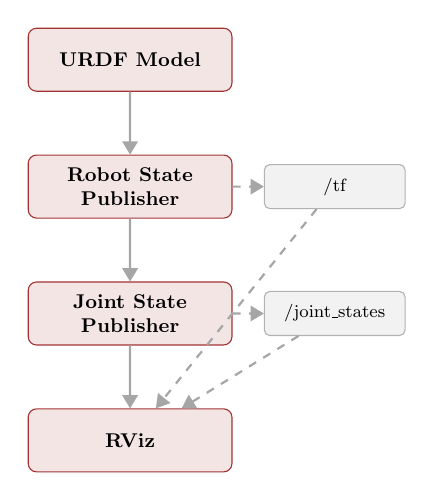
\begin{tikzpicture}[scale=0.8, transform shape, node distance=1cm]
        % RViz workflow
        \node[module, text width=3cm] (urdf) {URDF Model};
        \node[module, text width=3cm, below=of urdf] (rsp) {Robot State\\Publisher};
        \node[module, text width=3cm, below=of rsp] (jsp) {Joint State\\Publisher};
        \node[module, text width=3cm, below=of jsp] (rviz) {RViz};

        \draw[flow] (urdf) -- (rsp);
        \draw[flow] (rsp) -- (jsp);
        \draw[flow] (jsp) -- (rviz);

        % Topics
        \node[submodule, text width=2cm, right=0.5cm of rsp] (tf) {/tf};
        \node[submodule, text width=2cm, right=0.5cm of jsp] (js) {/joint\_states};

        \draw[flow, dashed] (rsp) -- (tf);
        \draw[flow, dashed] (jsp) -- (js);
        \draw[flow, dashed] (tf) -- (rviz);
        \draw[flow, dashed] (js) -- (rviz);
    \end{tikzpicture}
\end{column}
\end{columns}
\end{frame}

% ============================================
% SLIDE: Gazebo Simulation
% ============================================
\begin{frame}[shrink=3]{Gazebo Physics Simulation}
\begin{columns}
\begin{column}{0.5\textwidth}
    \textbf{Features:}
    \begin{itemize}
        \item Full physics simulation
        \item Collision detection
        \item Inertia-based dynamics
        \item World interaction
    \end{itemize}

    \vspace{0.3cm}

    \textbf{Launch Components:}
    \begin{enumerate}
        \item Empty world spawn
        \item TF footprint publisher
        \item Model spawner
        \item Fake joint calibration
    \end{enumerate}

    \vspace{0.3cm}

    \textbf{Usage:}
    \begin{itemize}
        \item \code{roslaunch Aloha gazebo.launch}
    \end{itemize}
\end{column}
\begin{column}{0.5\textwidth}
    \centering
    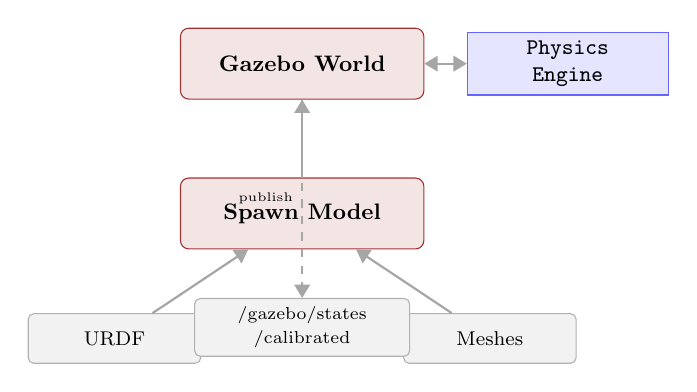
\begin{tikzpicture}[scale=0.9, transform shape, node distance=1.1cm]
        % Gazebo workflow
        \node[module, text width=3.2cm] (world) {Gazebo World};

        % Physics Engine
        \node[class, text width=2.6cm, right=0.6cm of world] (physics) {Physics\\Engine};
        \draw[flow, <->] (world) -- (physics);

        % Spawn Model
        \node[module, text width=3.2cm, below=of world] (spawn) {Spawn Model};
        \draw[flow] (spawn) -- (world);

        % URDF and Meshes
        \node[submodule, text width=2.2cm, below left=0.9cm and -0.3cm of spawn] (urdf) {URDF};
        \node[submodule, text width=2.2cm, below right=0.9cm and -0.3cm of spawn] (mesh) {Meshes};

        \draw[flow] (urdf) -- (spawn);
        \draw[flow] (mesh) -- (spawn);

        % Topics output
        \node[submodule, text width=2.8cm, below=2.8cm of world] (topics) {
            \scriptsize /gazebo/states\\
            \scriptsize /calibrated
        };
        \draw[flow, dashed] (world) -- node[left, font=\tiny] {publish} (topics);
    \end{tikzpicture}
\end{column}
\end{columns}
\end{frame}

% ============================================
% SLIDE: Directory Structure
% ============================================
\begin{frame}[fragile,shrink=3]{Directory Structure}
\begin{columns}
\begin{column}{0.5\textwidth}
\begin{lstlisting}[basicstyle=\ttfamily\tiny,numbers=none,frame=none]
simulation/src/Aloha/
+-- config/
|   +-- joint_names_Aloha.yaml
+-- launch/
|   +-- display.launch      # ROS1
|   +-- display.launch.py   # ROS2
|   +-- gazebo.launch
+-- meshes/
|   +-- base_link.STL
|   +-- wheel*.STL
|   +-- left_joint*.STL
|   +-- right_joint*.STL
+-- urdf/
|   +-- Aloha.urdf
+-- package.xml
\end{lstlisting}
\end{column}
\begin{column}{0.5\textwidth}
    \textbf{Mesh Files:}
    \begin{itemize}
        \item STL format (binary)
        \item SolidWorks export
        \item Collision \& visual
    \end{itemize}

    \vspace{0.2cm}

    \textbf{Build System:}
    \begin{itemize}
        \item ament\_cmake (ROS2)
        \item catkin (ROS1 compatible)
    \end{itemize}
\end{column}
\end{columns}
\end{frame}

% ============================================
% SLIDE: Module Summary
% ============================================
\begin{frame}{ROS Simulation Summary}
\begin{columns}
\begin{column}{0.5\textwidth}
    \textbf{Key Components:}
    \begin{itemize}
        \item URDF robot model
        \item STL mesh files
        \item ROS1/ROS2 launch files
        \item Joint configuration
    \end{itemize}

    \vspace{0.3cm}

    \textbf{Visualization:}
    \begin{itemize}
        \item RViz for visual inspection
        \item Joint state publisher GUI
        \item TF frame visualization
    \end{itemize}
\end{column}
\begin{column}{0.5\textwidth}
    \textbf{Physics Simulation:}
    \begin{itemize}
        \item Gazebo integration
        \item Inertia-based dynamics
        \item Collision meshes
    \end{itemize}

    \vspace{0.3cm}

    \textbf{Comparison with ManiSkill3:}
    \begin{table}
    \centering
    \footnotesize
    \begin{tabular}{lcc}
    \toprule
    \textbf{Feature} & \textbf{ROS} & \textbf{ManiSkill3} \\
    \midrule
    Physics & Gazebo & SAPIEN \\
    GPU Accel & No & Yes \\
    RL Support & Limited & Native \\
    Visualization & RViz & Viewer \\
    \bottomrule
    \end{tabular}
    \end{table}
\end{column}
\end{columns}
\end{frame}



% ============================================
% APPENDIX: DIRECTORY STRUCTURE
% ============================================

\appendix

\section{Appendix}

\begin{frame}[fragile]{Directory Structure}
\begin{columns}
\begin{column}{0.5\textwidth}
\begin{lstlisting}[basicstyle=\ttfamily\tiny,numbers=none,frame=none]
AlohaMini/
+-- docs/           # Documentation
+-- hardware/       # CAD files
+-- maniskill/      # ManiSkill3
|   +-- agents/     # Robot agents
|   +-- teleop/     # Teleoperation
|   +-- assets/     # URDF/meshes
|   +-- examples/   # Demo scripts
+-- software/       # LeRobot
+-- simulation/     # ROS packages
\end{lstlisting}
\end{column}
\begin{column}{0.5\textwidth}
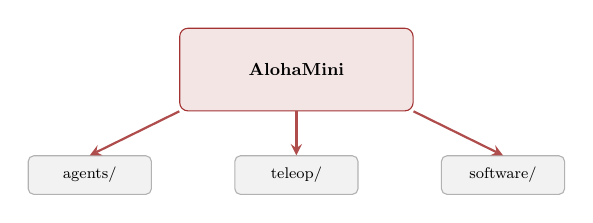
\begin{tikzpicture}[scale=0.7, transform shape]
    % Main box
    \node[module, text width=4cm, minimum height=1.5cm] (main) at (0,0) {AlohaMini};

    % Sub modules
    \node[submodule, below left=0.8cm and 0.5cm of main] (agents) {agents/};
    \node[submodule, below=0.8cm of main] (teleop) {teleop/};
    \node[submodule, below right=0.8cm and 0.5cm of main] (software) {software/};

    % Arrows
    \draw[arrow] (main.south west) -- (agents.north);
    \draw[arrow] (main.south) -- (teleop.north);
    \draw[arrow] (main.south east) -- (software.north);
\end{tikzpicture}
\end{column}
\end{columns}
\end{frame}

\begin{frame}{Module Dependencies}
\centering
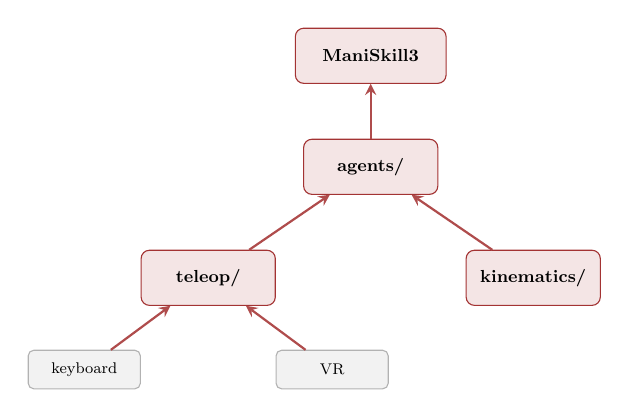
\begin{tikzpicture}[node distance=1cm, scale=0.7, transform shape]
    % Top level
    \node[module, text width=2.5cm] (maniskill) {ManiSkill3};

    % Second level
    \node[module, text width=2.2cm, below=of maniskill] (agents) {agents/};

    % Third level
    \node[module, text width=2.2cm, below left=1cm and 0.5cm of agents] (teleop) {teleop/};
    \node[module, text width=2.2cm, below right=1cm and 0.5cm of agents] (kinematics) {kinematics/};

    % Fourth level
    \node[submodule, text width=1.8cm, below left=0.8cm and 0cm of teleop] (keyboard) {keyboard};
    \node[submodule, text width=1.8cm, below right=0.8cm and 0cm of teleop] (vr) {VR};

    % Arrows
    \draw[arrow] (agents) -- (maniskill);
    \draw[arrow] (teleop) -- (agents);
    \draw[arrow] (kinematics) -- (agents);
    \draw[arrow] (keyboard) -- (teleop);
    \draw[arrow] (vr) -- (teleop);
\end{tikzpicture}
\end{frame}

% Final slide
\begin{frame}
\centering
\vspace{2cm}
{\Huge\color{darkred} Thank You}

\vspace{1cm}

{\large AlohaMini Codebase Documentation}

\vspace{0.5cm}

\url{https://github.com/AlohaMini}
\end{frame}

\end{document}
